% This is a LaTeX template kindly taken from Jernej Debevec.
% Provided by Miha Muskinja for the purpose of the seminar I in the 1st year
% of the 2nd cycle of the study of physics at the Faculty of Mathematics and Physics, University of Ljubljana.

% Set the document class and options
\documentclass[10pt, titlepage, a4paper]{article}
\usepackage[a4paper, inner=2.5cm, outer=2.5cm, top=2.25cm, bottom=2.25cm]{geometry}
\usepackage{graphicx}
\usepackage{hyperref}
\usepackage{wrapfig}
\usepackage{amsfonts}
\usepackage{amsmath}
\usepackage{bbm}
\usepackage{float}
\usepackage{xfrac}
\hypersetup{colorlinks=true}

% Load the natbib package for citation style
\usepackage{natbib}

% Some macros for commonly used symbols in physics/quantum mechanics
\newcommand{\bb}[1]{\mathbf#1}
\newcommand{\dd}{\mathrm{d}}
\newcommand{\pp}{\partial}
\newcommand{\dg}{\dagger}
\newcommand{\la}{\langle}
\newcommand{\ra}{\rangle}
\newcommand{\id}{\mathbb{1}}
\newcommand{\T}{\mathsf{T}}
\newcommand{\ua}{\uparrow\>}
\newcommand{\da}{\downarrow\>}
\newcommand{\fs}[1]{\slashed{#1}}  % Feynmann slash
\newcommand{\mc}[1]{\mathcal{#1}}
\newcommand\thickbar[1]{\accentset{\rule{.5em}{.03em}}{#1}}
\renewcommand{\bar}{\thickbar}

% Start the document
\begin{document}

% The title page
\begin{titlepage}
{\centering

\includegraphics[width=6cm]{logo_fmf.pdf}

\vspace{0.8cm}
{\small Department of Physics}

\vspace{5cm}
\vspace{0.5cm}
{\huge\textbf{Time Series Analysis using Auto Regressive models}} \\
\vspace{0.5cm}
{\large\textbf{12. Task for Model Analysis I, 2023/24}}

\vfill
\textbf{Author:} Marko Urbanč \\
\textbf{Professor:} Prof. dr. Simon Širca  \\ 
\textbf{Advisor:}  doc. dr. Miha Mihovilovič \\

\vspace{1cm}
Ljubljana, August 2024 \\
}
\vspace{3cm}
\end{titlepage}

% Add table of conents
\hypersetup{pageanchor=true}
\pagenumbering{roman}
\setcounter{page}{2}
\tableofcontents
\vspace{1cm}

% Proceed with the main body
\pagenumbering{arabic}

% Sections based on typical Model Analysis structure
\section{Introduction}
In physics we often encounter time series data as we measure the evolution of a system in time. Today we'll be having 
a look at one of the plethora of methods in our time series analysis arsenal, called Auto Regressive (AR) models. Then 
we'll apply this method to a few different datasets to study its performance, applicability and behavior. AR models are 
a class of linear models that predict the future values of a time series based on its past values. Based on the 
coefficients of the model, we can infer the underlying dynamics of the system or find the signals spectrum. \\

An AR model of order $p$ is defined as:
%
\begin{equation}
    X_t = \sum_{i=1}^p a_i X_{t-i} + \epsilon_t\>,
\end{equation}
%
where $X_t$ is the time series at time $t$, $a_i$ are the coefficients of the model and $\epsilon_t$ is the error term which 
we assume to be uncorrelated and with zero mean. In our idealized case, we'll only have a short look at how noise 
affects the model. For the coefficients $a_i$ we can without loss of generality divide by the first coefficient, $a_1$,
which yields a model with a leading coefficient of 1. The order of the model, $p$, is a hyperparameter that determines 
how many past values of the time series we use to predict the future value. The model is commonly used in the context of 
machine learning but today we'll be solving for the coefficients more hands-on, with out explicit use of optimization 
algorithms. \\

A popular method to determine the AR model coefficients are the Yule-Walker equations. These are a set of $p$ linear
equations that can be solved for the coefficients which are given by the autocorrelation of the time series 
$\{X_t\}$. The autocorrelation is defined as:
%
\begin{equation}
    r_n = \sum_{i=1}^p a_i r_{n-i}\>,
\end{equation}
%
where $r_n$ is the autocorrelation at lag $n$. Essentially we need to solve a Toeplitz system of equations. The 
system of equations is given by:
%
\begin{equation}~
    \rm{R} \bb{a} = \bb{r}\>,
\end{equation}
%
where $\rm{R}$ is the autocorrelation matrix, given as:
%
\begin{equation}
    \rm{R} = \begin{bmatrix}
        r_0 & r_1 & \cdots & r_{p-1} \\
        r_1 & r_0 & \cdots & r_{p-2} \\
        \vdots & \vdots & \ddots & \vdots \\
        r_{p-1} & r_{p-2} & \cdots & r_0
    \end{bmatrix}\>,
\end{equation}
%
and $\bb{r}$ and $\bb{a}$ are the autocorrelation vector and coefficient vector respectively, given as:
%
\begin{equation}
    \bb{r} = \begin{bmatrix}
        r_1 \\
        r_2 \\
        \vdots \\
        r_p
    \end{bmatrix}\quad\quad\text{and}\quad\quad
    \bb{a} = \begin{bmatrix}
        a_1 \\
        a_2 \\
        \vdots \\
        a_p
    \end{bmatrix}\>.
\end{equation}
%
Stability of the model is ensured by the roots of the characteristic polynomial of the model which must 
lie inside the unit circle on the complex plane. This is something we'll have to keep in mind when analyzing the
results, as any roots outside the unit circle will make the model unstable. \\

\section{Task}
\subsection{Spectra of Signals}
The instructions want us to plot the spectra of a few different signals that have been provided. The main comparison 
should be between the spectra given by the AR model and the spectra given by the Fourier transform. The FFT algorithm 
is truly a marvel of modern mathematics and computing so it will definitely be a tough competitor. The signals that have 
been provided are plotted in Figure \ref{fig:signals}.

\begin{figure}[H]
    \centering
    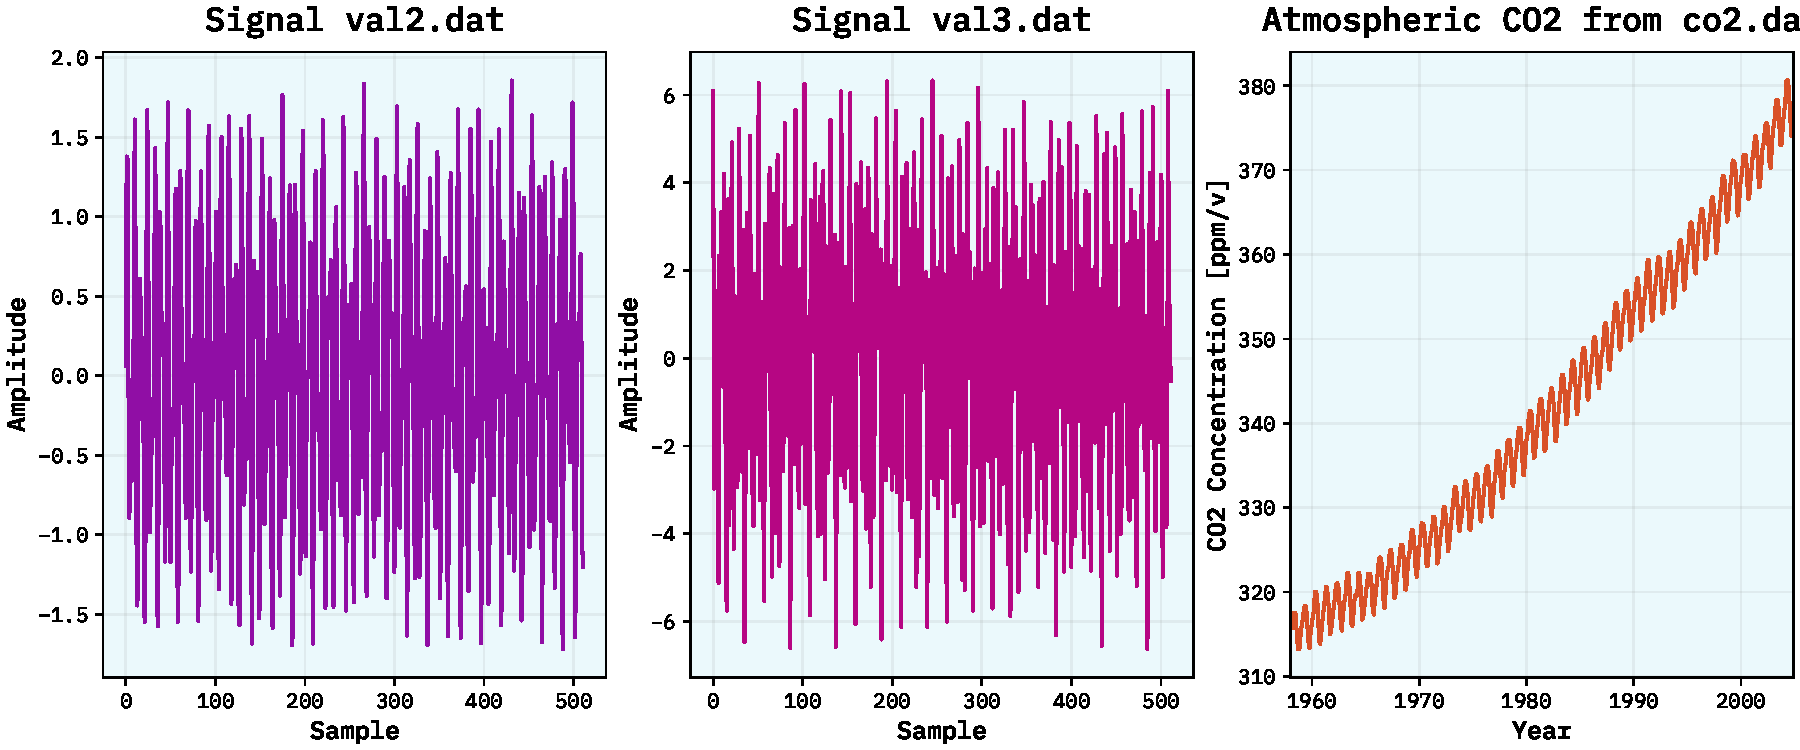
\includegraphics[width=0.95\textwidth]{../MaxEntropy/Images/supplied-data.pdf}
    \caption{The signals that we'll be analyzing in the first subtask.}
    \label{fig:signals}
\end{figure}

The instructions also want us to explore the various properties of the AR model and how it behaves when we change the
order of the model as well as the number of points we use to evaluate the spectra. The spectra can be calculated 
using the following formula:
%
\begin{equation}
    S(f) = \frac{1}{|1 - \sum_{i=1}^p a_i e^{-2\pi i f i}|^2}\>,
\end{equation}
%
however I used the \texttt{scipy.signal.freqz} for ease of use and to avoid any mistakes. For anyone interested further 
this article by Emanuel Parzen \cite{parzen} goes more in depth. 

\subsection{Forecasting Signals}
In the second subtask we've been provided some additional signals that we'll be using in combination with the signals from 
the first subtask to study the performance of the AR model in forecasting. The supplied signals are plotted in Figure 
\ref{fig:signals-2}.

\begin{figure}[H]
    \centering
    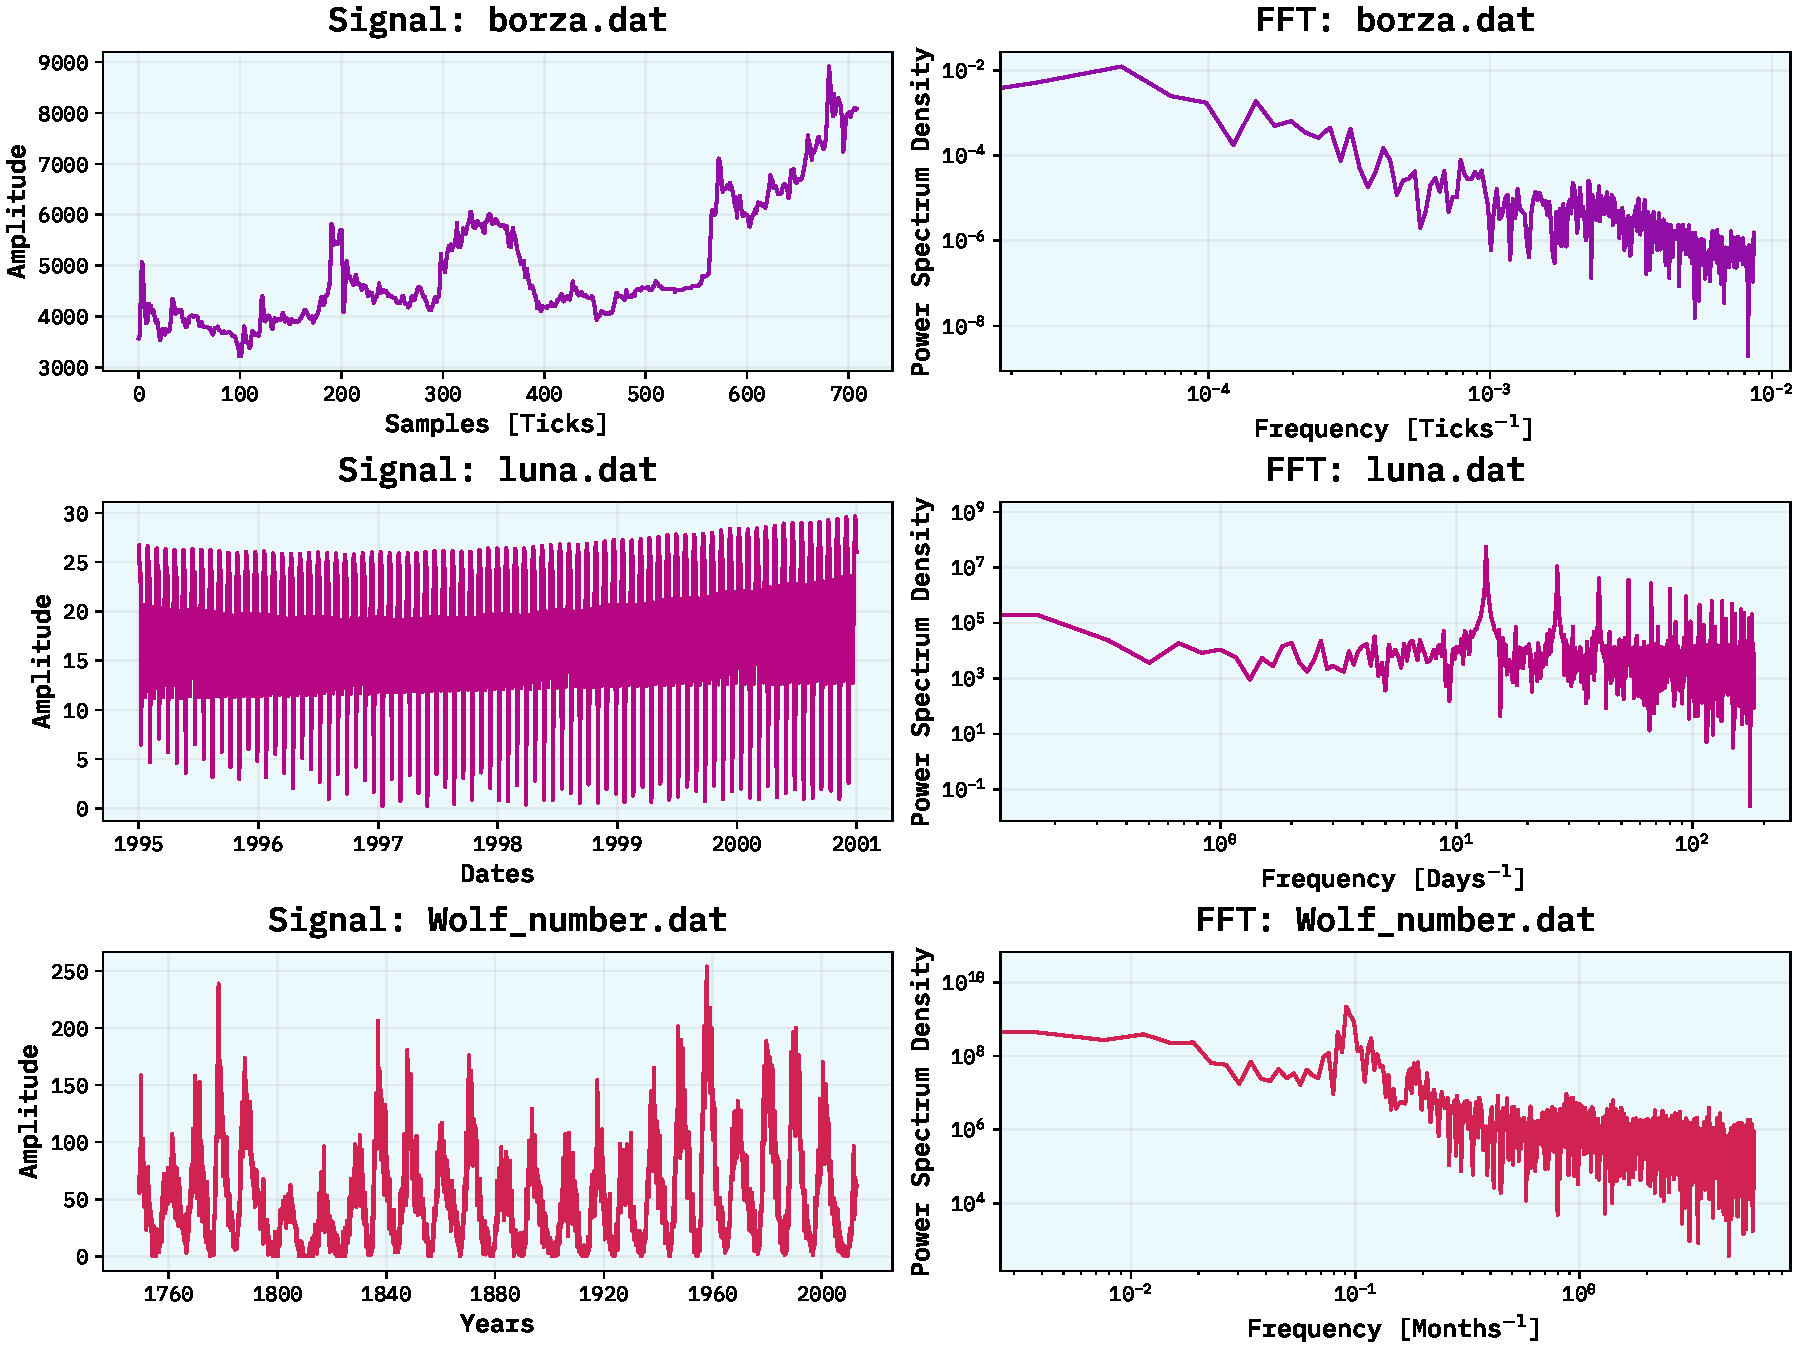
\includegraphics[width=0.95\textwidth]{../LinForecast/Images/new-data.pdf}
    \caption{The signals that we'll be adding to our analysis in the second subtask.}
    \label{fig:signals-2}
\end{figure}

They represent a stock's value, ephemeris data for the moon and Wolf sunspot numbers. The instructions want us to
forecast the signals using the AR model and compare the results with the actual data. We can do so by providing half 
of the data to the model and then comparing the forecasted values with the actual values of the other half. We should also 
have a look at how noise affects the model and the forecasted values.

\section{Solution Overview}
Due to my speedrunning of these tasks this task lacks any extra bells and whistles. I implemented the Yule-Walker 
method using \texttt{numpy} and \texttt{scipy} by making a class \texttt{YuleWalker} that can be used to fit the 
model and evaluate PSDs. It takes inputs of the time series and the order of the model. I really like classes in Python.
They really serve well as containers for variables and their associated functions. The class also has a method to
forecast the time series using the AR model. The results are presented in the following sections. Before we proceed 
we need to detrend some of the signals. This was most commonly done by subtracting the mean of the signal, however I 
encountered two special cases. The first was the CO2 atmospheric concentration signal to which I fit a square 
polynomial and subtracted the fit from the signal. The second signal was the stock value signal which I detrended by
the linear fit of the signal. The signals with their respective trends are plotted in Figures \ref{fig:detrended-1} 
and \ref{fig:detrended-2}.

\begin{figure}[H]
    \centering
    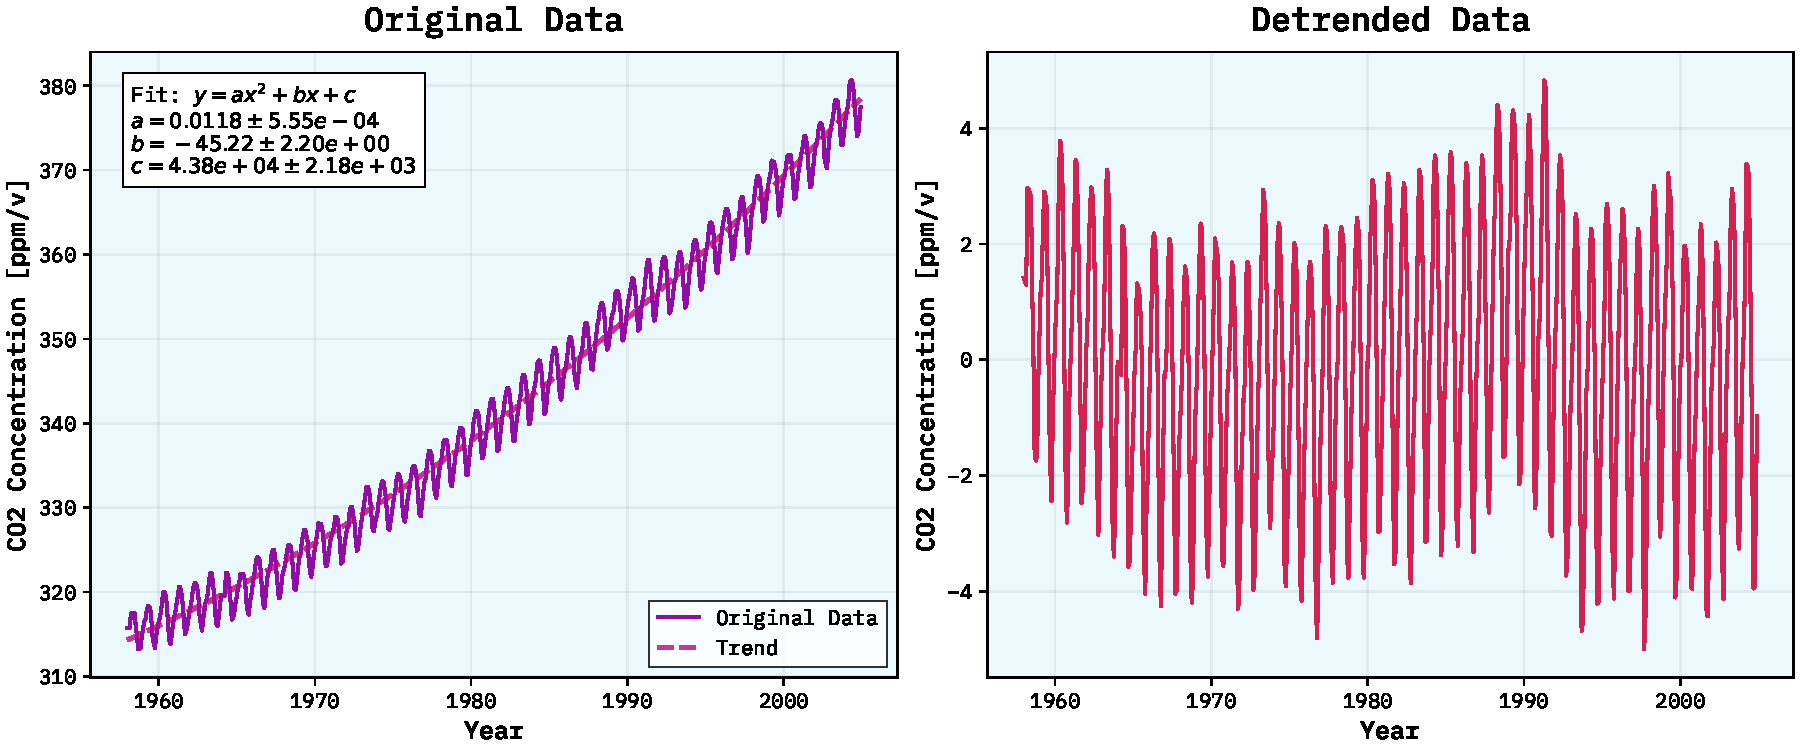
\includegraphics[width=0.95\textwidth]{../MaxEntropy/Images/detrended-co2.pdf}
    \caption{The CO2 atmospheric concentration signal with a square polynomial fit.}
    \label{fig:detrended-1}
\end{figure}

\begin{figure}[H]
    \centering
    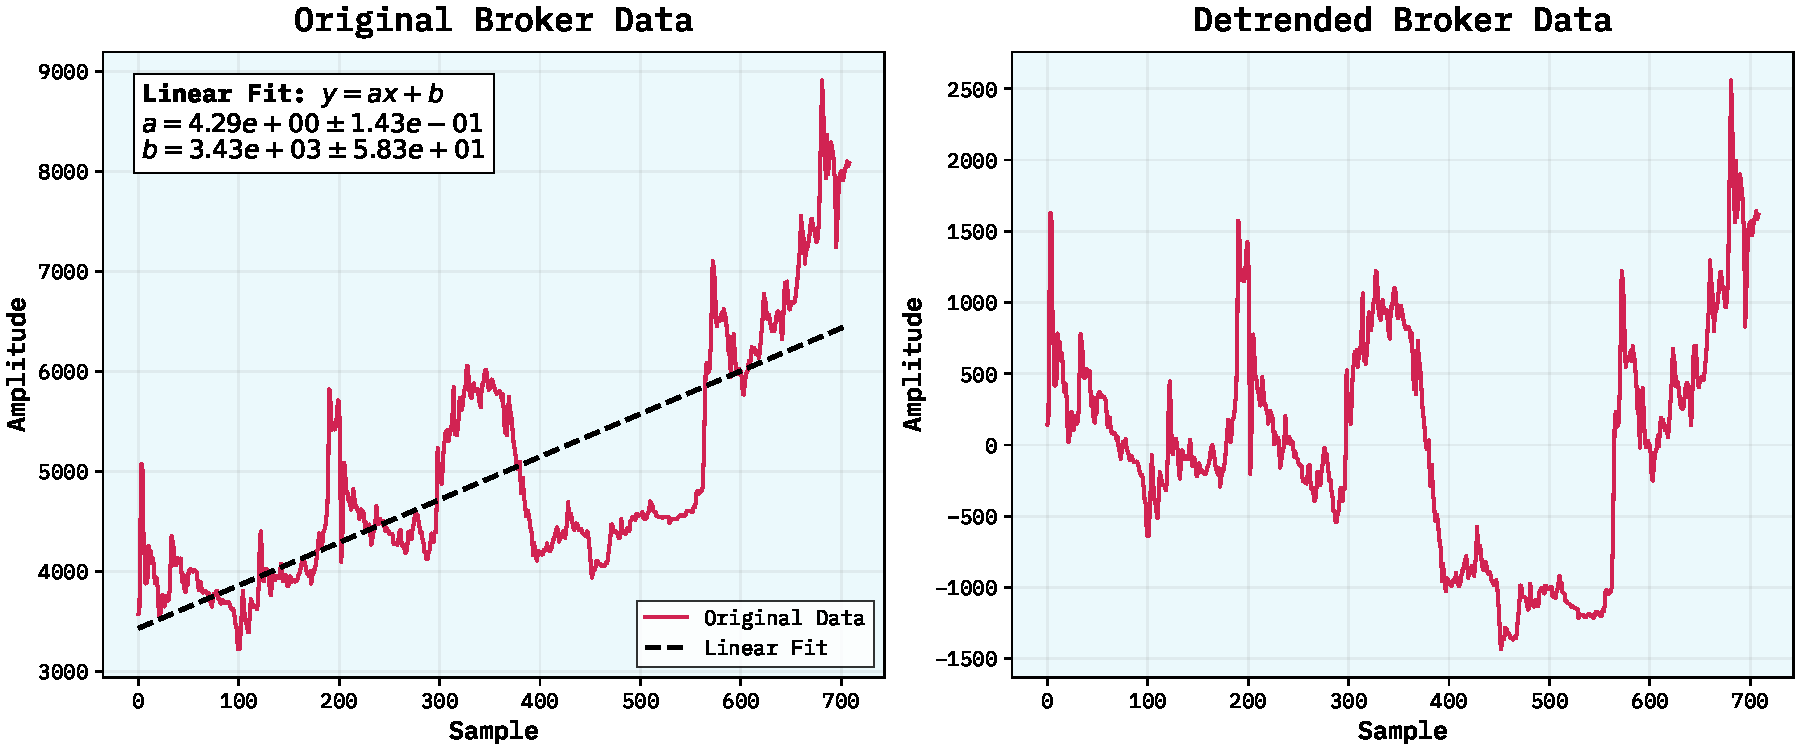
\includegraphics[width=0.95\textwidth]{../LinForecast/Images/borza-detrended.pdf}
    \caption{The stock value signal with a linear fit.}
    \label{fig:detrended-2}
\end{figure}

\section{Results}
\subsection{Spectra of Signals}
As described above I used the \texttt{scipy.signal.freqz} function to evaluate the spectra of the signals. The results 
are plotted in Figures \ref{fig:spectra-1}, \ref{fig:spectra-2} and \ref{fig:spectra-3}. The AR model seems to do a 
fantastic job at approximating the spectra of the signals. The absolute scale of the spectra are larger than expected however 
they match up relatively well with the FFT spectra. What is definitely visible are the wider peaks in the AR model spectra 
compared to the FFT spectra. I think it makes sense to study the width of the peaks a bit more in depth.

\begin{figure}[H]
    \centering
    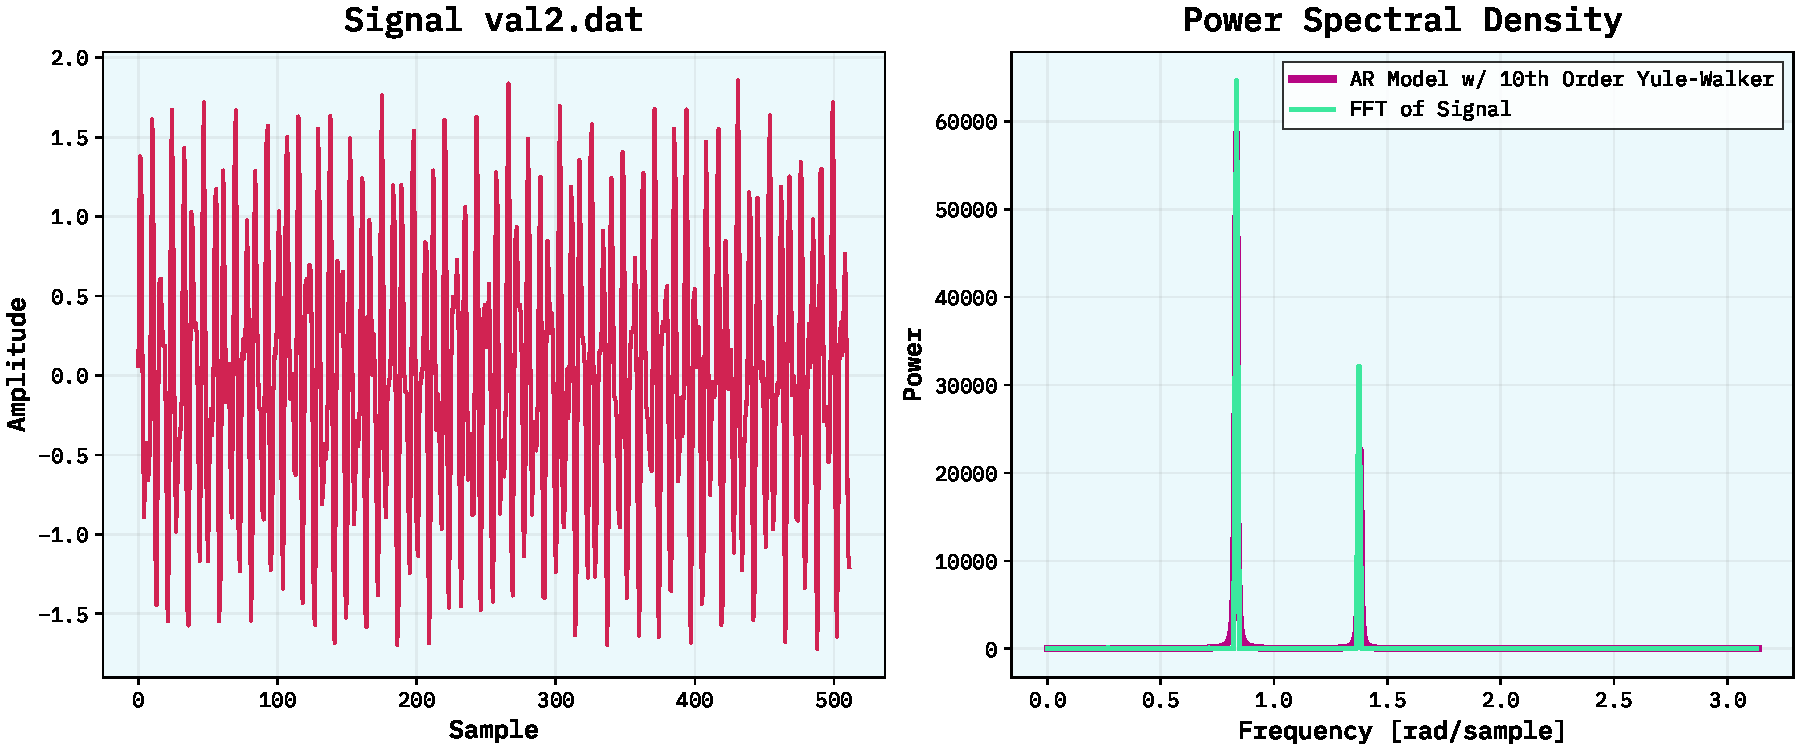
\includegraphics[width=0.95\textwidth]{../MaxEntropy/Images/yw-demo-val2.dat.pdf}
    \caption{The spectra signal \texttt{val2.dat}.}
    \label{fig:spectra-1}
\end{figure}

\begin{figure}[H]
    \centering
    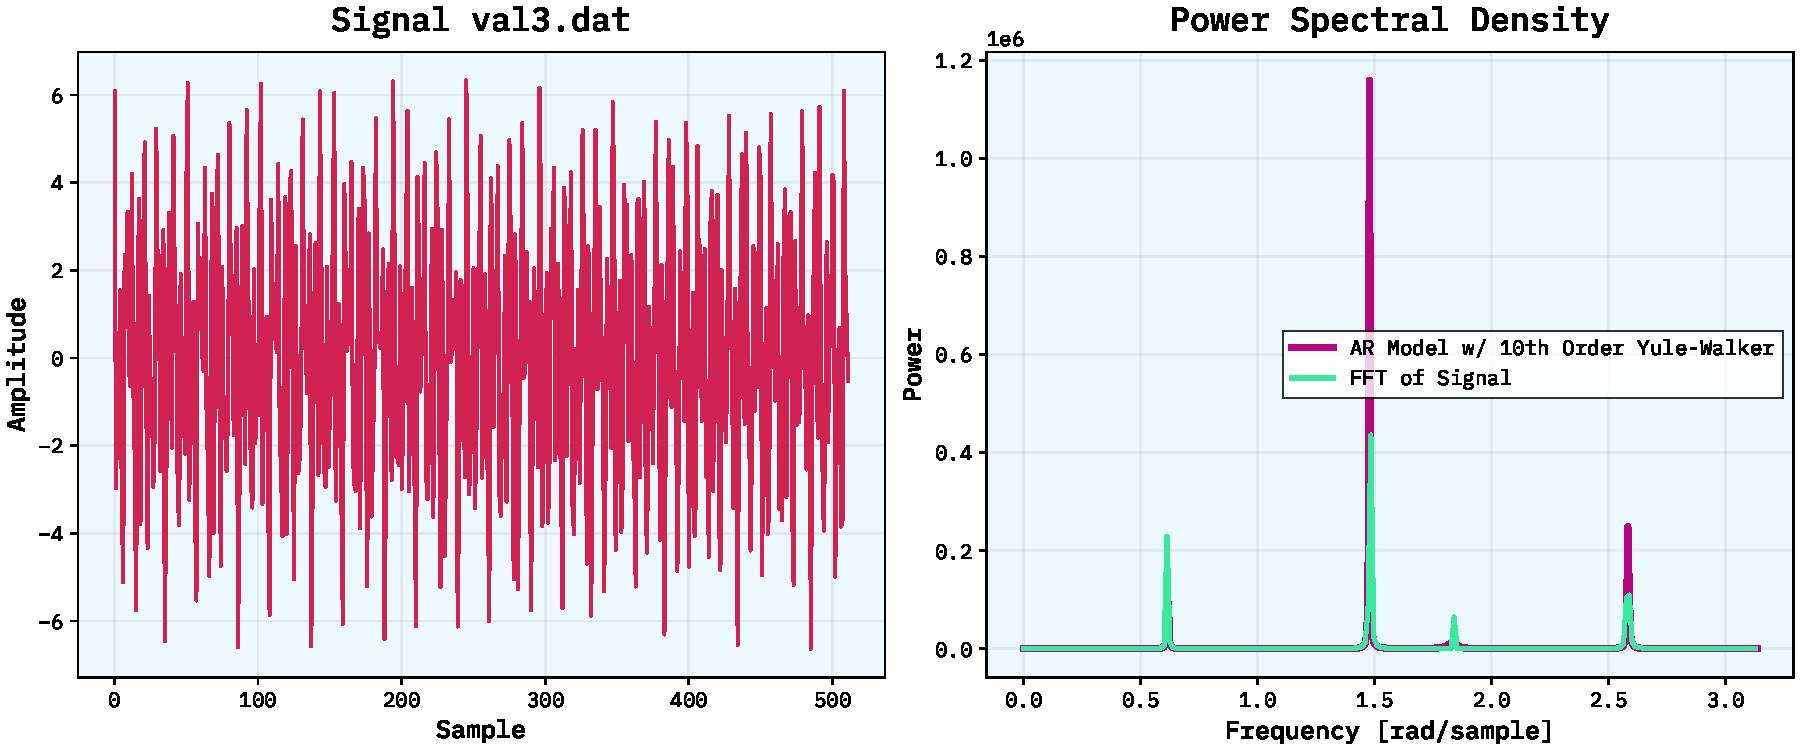
\includegraphics[width=0.95\textwidth]{../MaxEntropy/Images/yw-demo-val3.dat.pdf}
    \caption{The spectra signal \texttt{val3.dat}.}
    \label{fig:spectra-2}
\end{figure}

\begin{figure}[H]
    \centering
    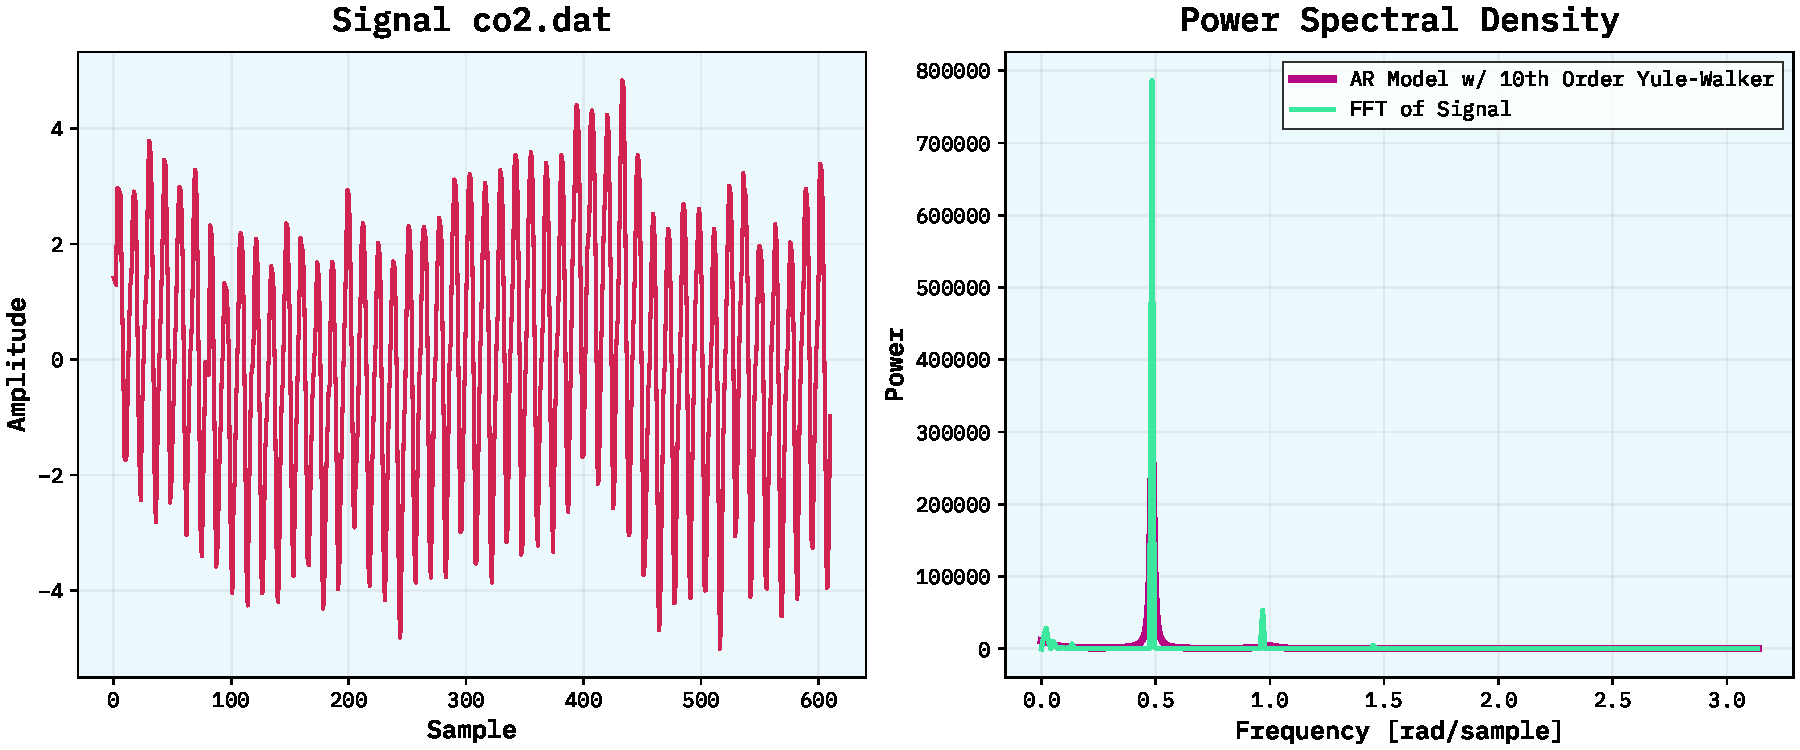
\includegraphics[width=0.95\textwidth]{../MaxEntropy/Images/yw-demo-co2.dat.pdf}
    \caption{The spectra signal \texttt{co2.dat}.}
    \label{fig:spectra-3}
\end{figure}

As stated above lets have a look at the width of peaks in the spectra. I evaluated the widths with the help of 
\texttt{scipy.signal.find\_peaks} and \texttt{scipy.signal.peak\_widths} on signals \texttt{val2.dat} and \texttt{val3.dat}.
The results are plotted in Figures \ref{fig:width-1} and \ref{fig:width-2}. Plotted alongside are also the roots of the 
characteristic polynomial for each model.

\begin{figure}[H]
    \centering
    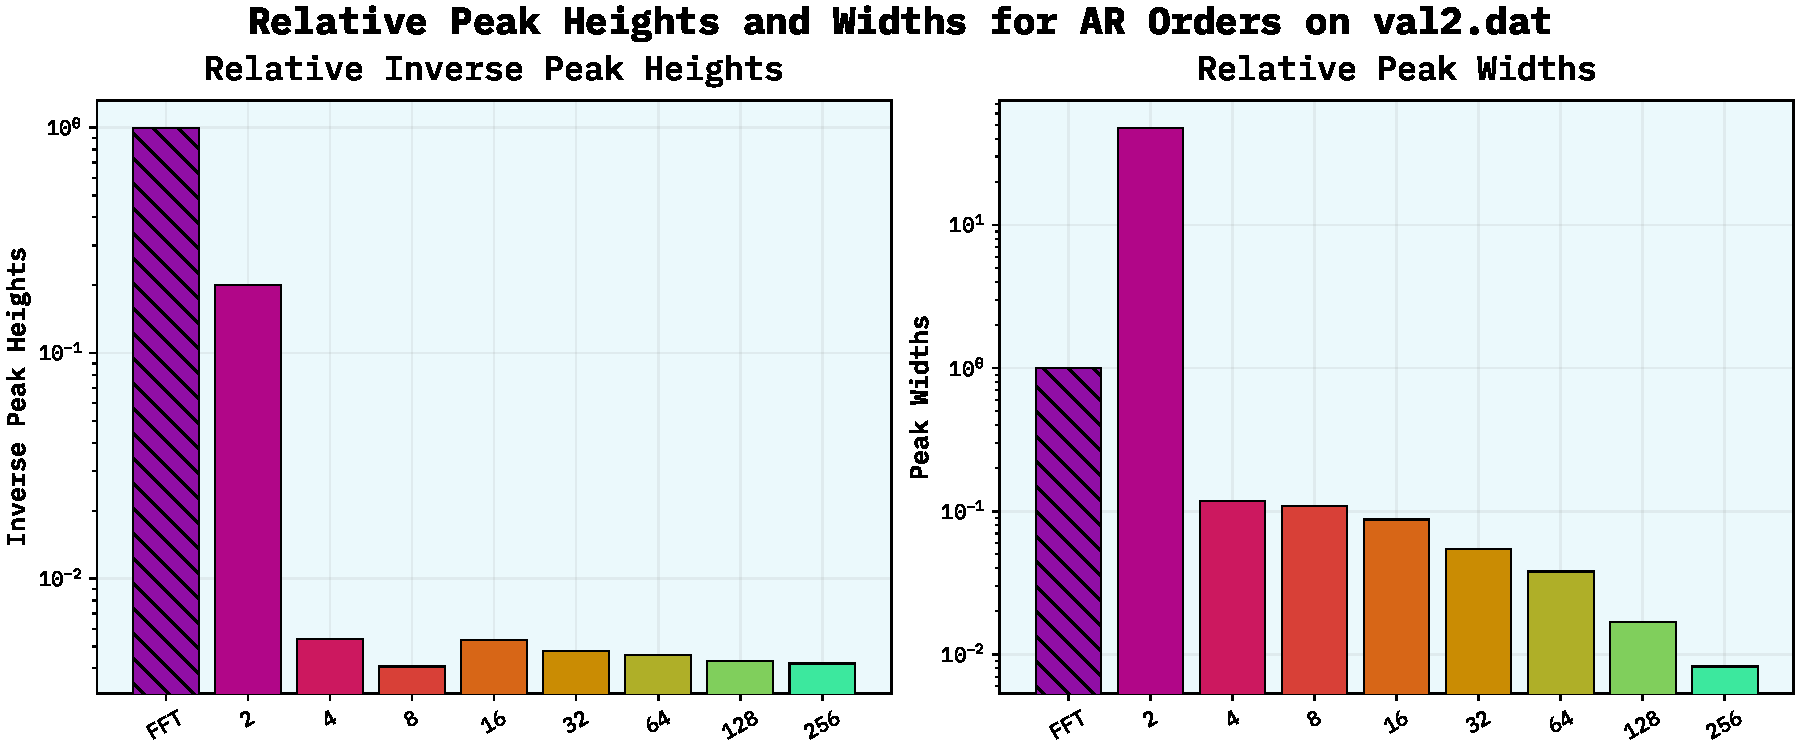
\includegraphics[width=0.95\textwidth]{../MaxEntropy/Images/peak-widths-val2.dat.pdf}
    \caption{The peak widths/heights of the spectra of signal \texttt{val2.dat}.}
    \label{fig:width-1}
\end{figure}

\begin{figure}[H]
    \centering
    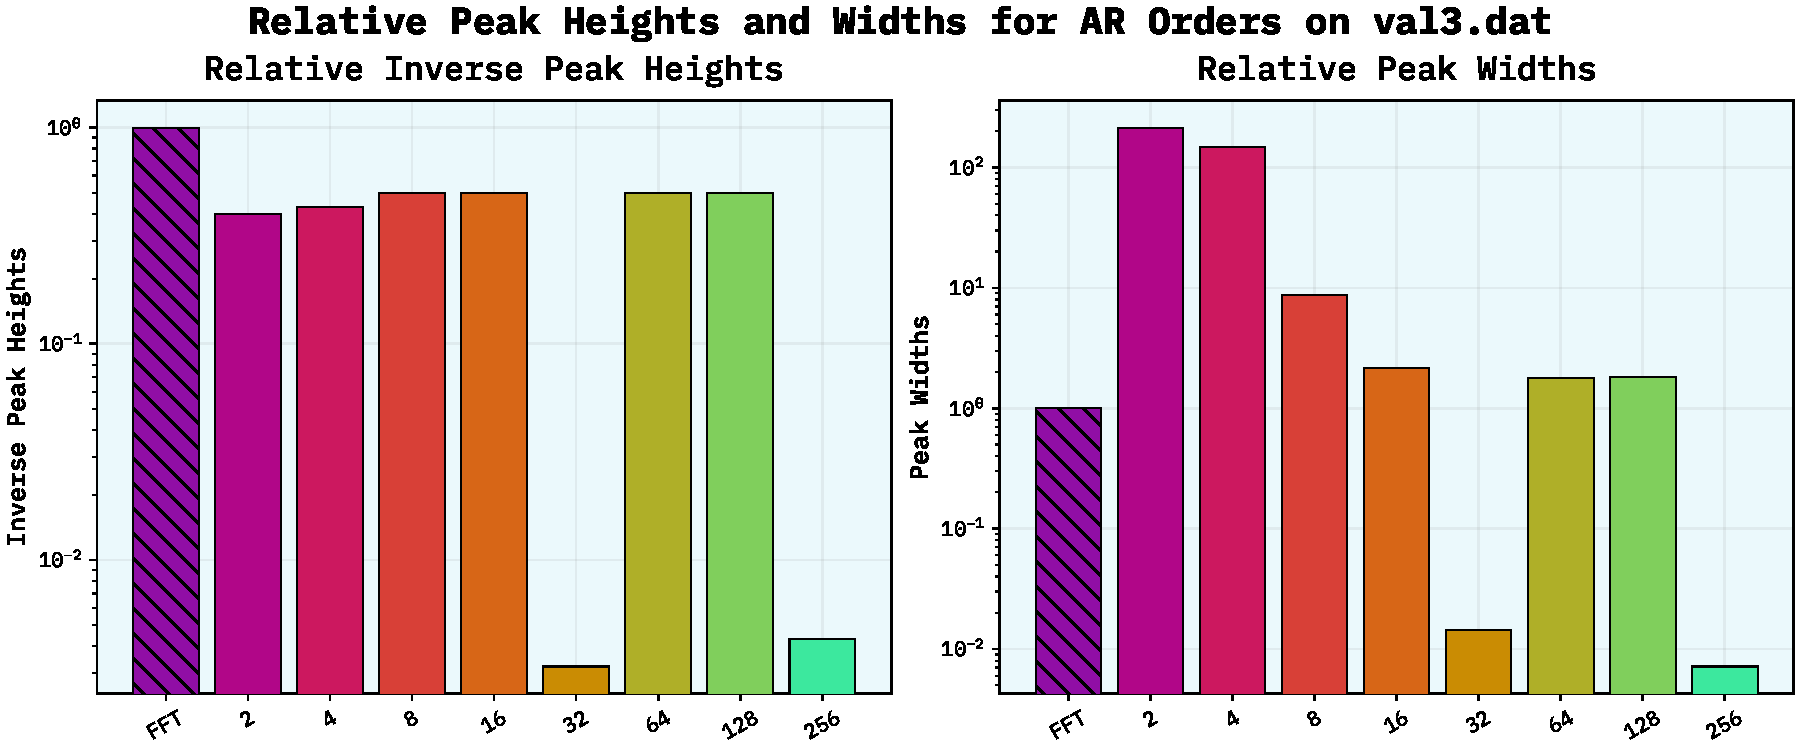
\includegraphics[width=0.95\textwidth]{../MaxEntropy/Images/peak-widths-val3.dat.pdf}
    \caption{The peak widths/heights of the spectra of signal \texttt{val3.dat}.}
    \label{fig:width-2}
\end{figure}

These plots are a bit more information dense so it makes sense to give some explanation. The left-most plot shows the relative 
inverse peak height as compared to the FFT spectra. The inverse height meaning that the values plotted present 
$\frac{1}{\text{height}}$. This was done due to a massive range in the heights of the peaks which generally depend on the order 
of the filter as we can also see from the plot. There seems to be a relatively steady downwards trend in the inverse peak height, which 
means that they are growing. A similar trend can be seen in the middle subplot which represents the relative peak widths. Do note, that 
there is no inverse in play here. We can see that the widths of the peaks narrow as the order of the AR model rises. For low 
values of the AR model order the peaks are much wider than the FFT peaks. In fact they more resemble bumps rather than 
sharp peaks. The right-most plot shows the roots of the characteristic polynomial of the AR model. The main focus here was to check 
that all of the roots are inside the unit circle which is also plotted. The roots seem to be stable. I find the way the roots spread around 
in the complex plane incredibly fascinating. \\

For a better comparison between the AR model and the FFT spectra I plotted all the spectra on the same plot. Do note here that 
the AR and FFT spectra have been normalized such that we look at relative differences in scale, not absolute. The result 
is presented in Figure \ref{fig:all-spectra}.

\begin{figure}[H]
    \centering
    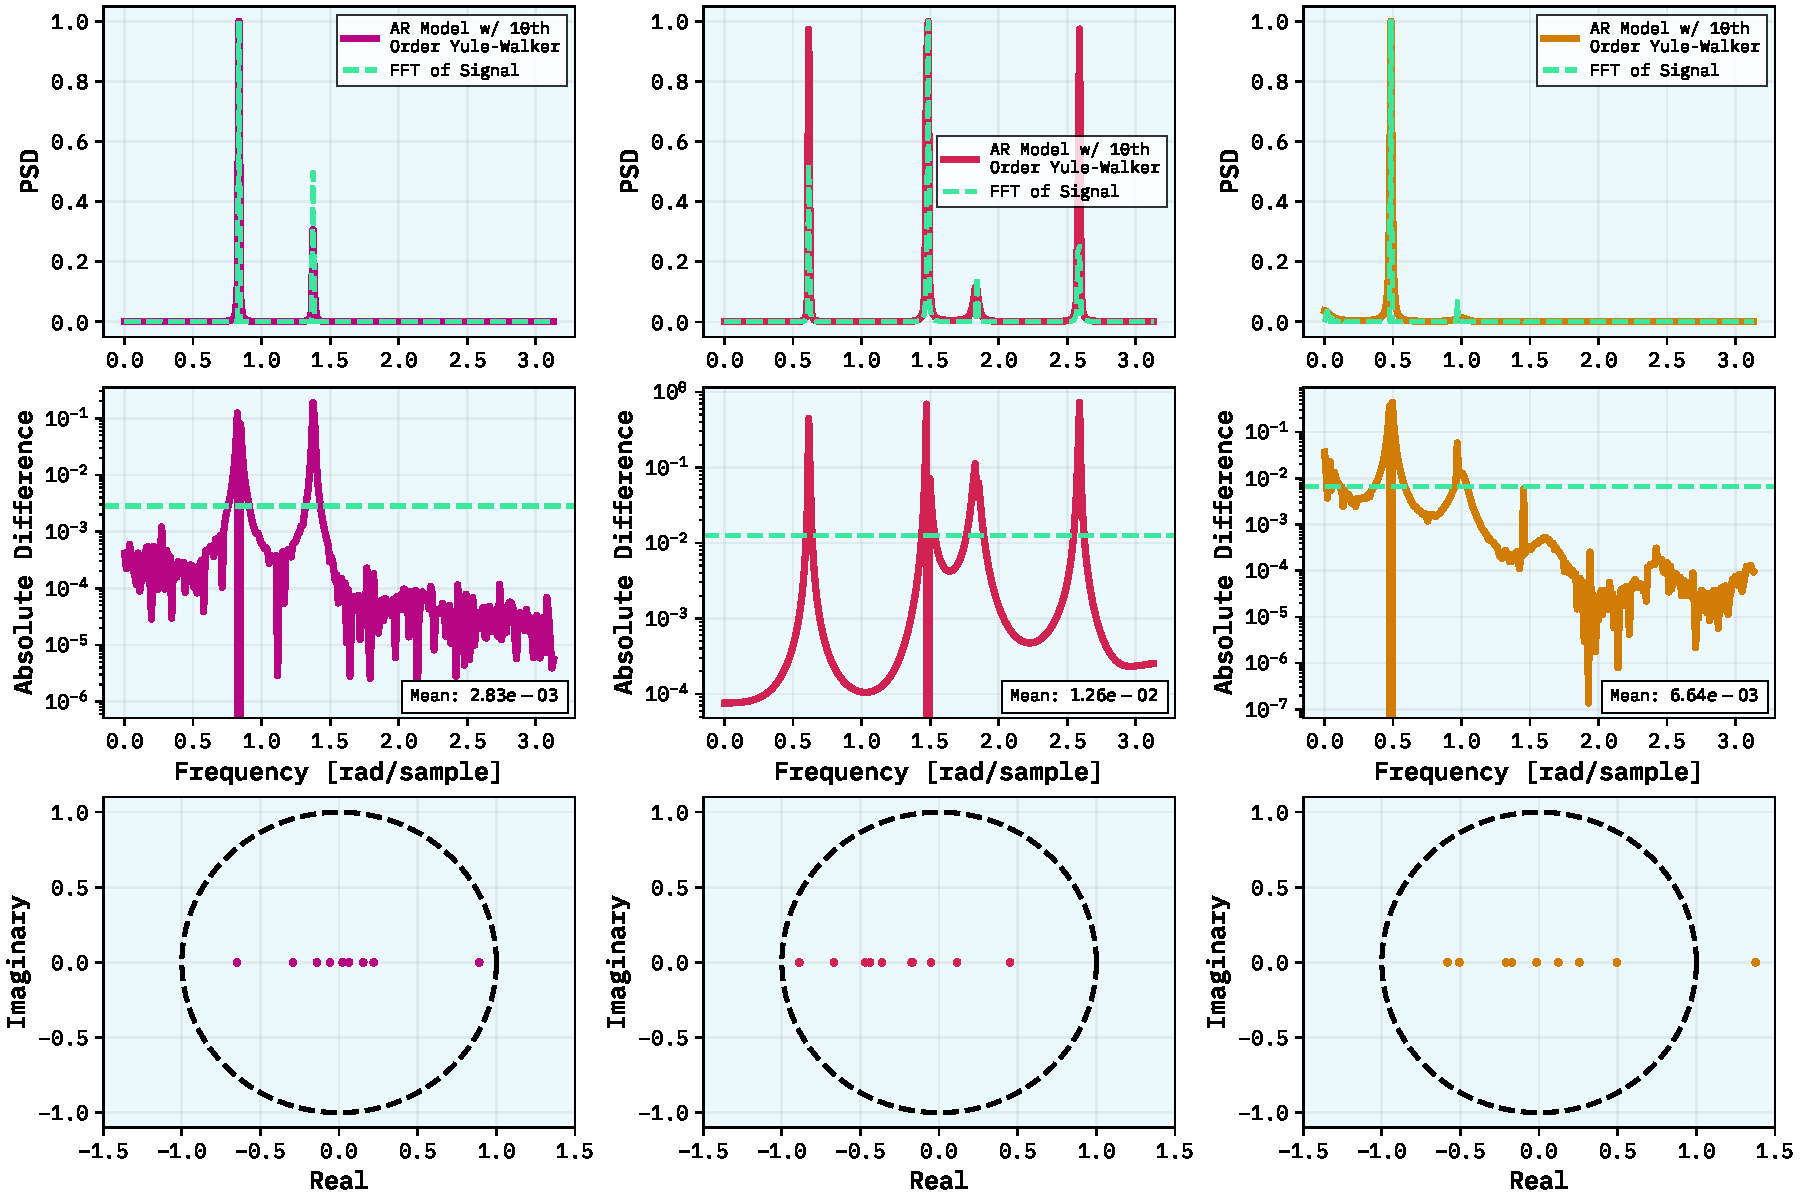
\includegraphics[width=0.95\textwidth]{../MaxEntropy/Images/fft-ar-model-compare.pdf}
    \caption{All the spectra of the signals on the same plot.}
    \label{fig:all-spectra}
\end{figure}

Again for the sense of safety and to check our methods I've also included the roots of the polynomials on the same plot.
I'd like the reader to note that the AR models are not of the same order. The AR model order was chosen based on what I felt 
empiricaly gave the best results. We see that the spectra line up very nicely. There are some differences but we can see 
that for all the provided signals the mean absolute error is in the order of $10^{-3}$. \\ 

Lastly lets have a look at the effects filter order and number of evaluation points (evaluation density) have on the
spectra. This time I've also included \texttt{co2.dat} in the analysis. The results are plotted in Figures 
\ref{fig:order-1}, \ref{fig:order-2} and \ref{fig:order-3}. 

\begin{figure}[H]
    \centering
    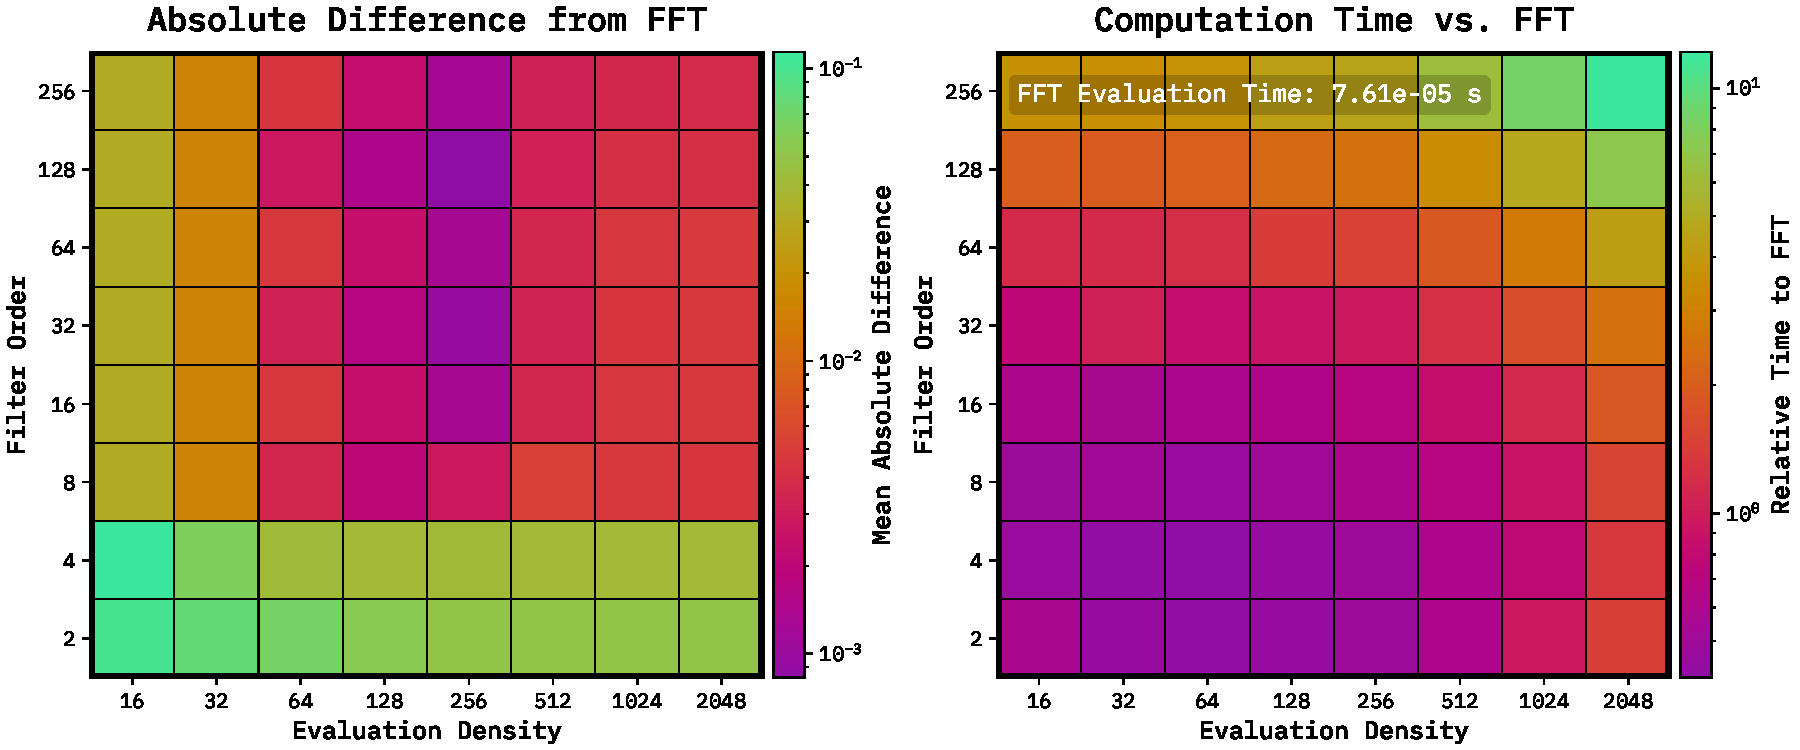
\includegraphics[width=0.95\textwidth]{../MaxEntropy/Images/order-density-val2.dat.pdf}
    \caption{The effects of filter order and evaluation density on the spectra of signal \texttt{val2.dat}.}
    \label{fig:order-1}
\end{figure}

\begin{figure}[H]
    \centering
    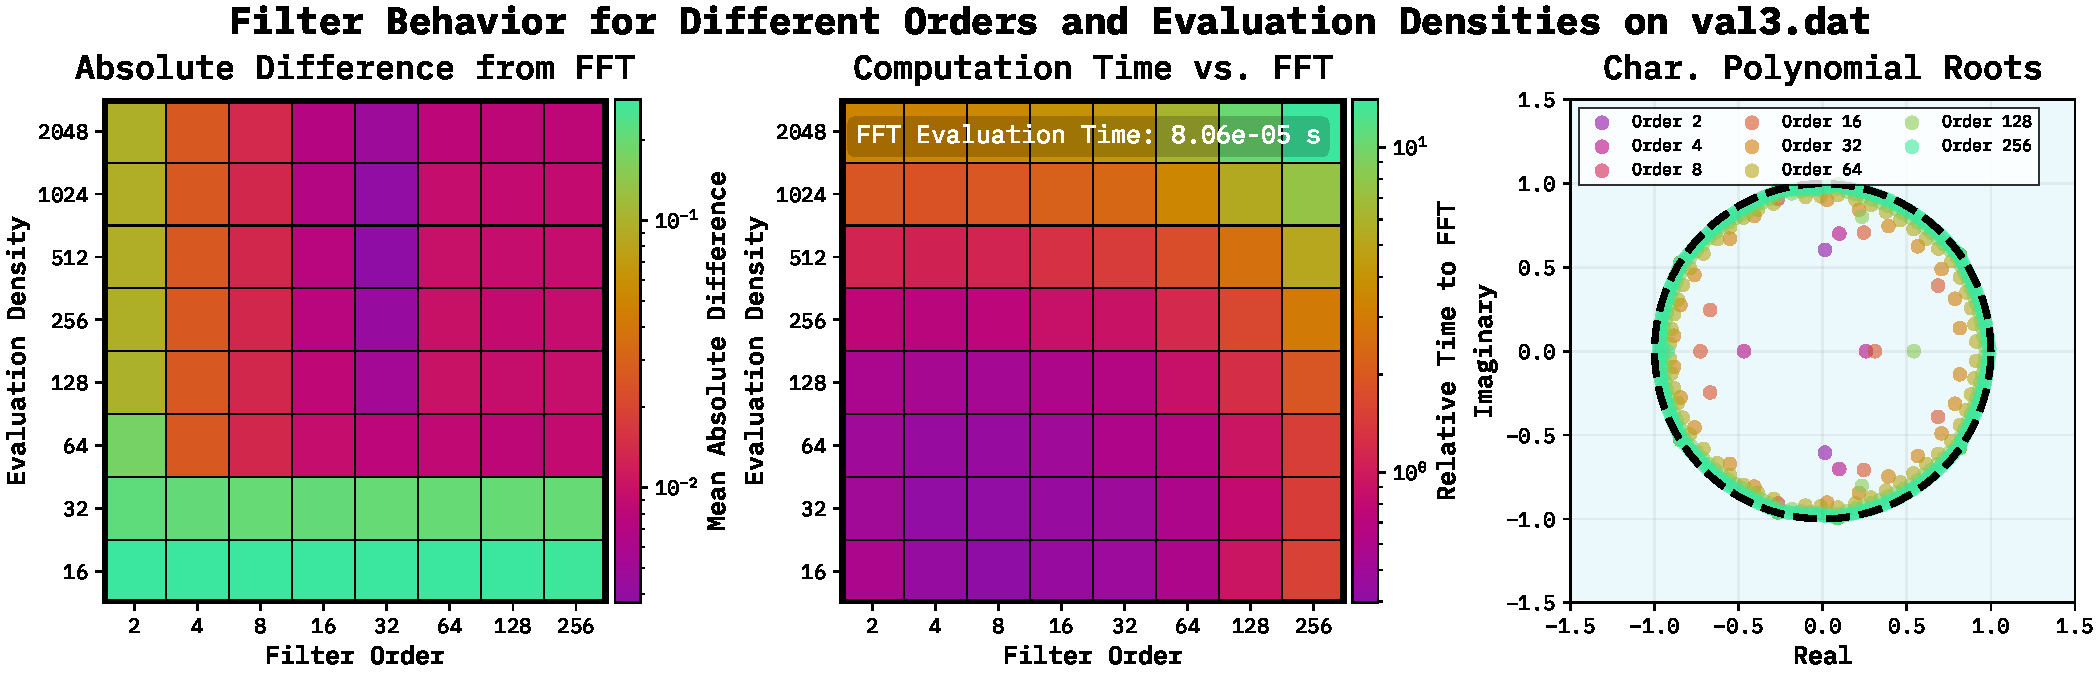
\includegraphics[width=0.95\textwidth]{../MaxEntropy/Images/order-density-val3.dat.pdf}
    \caption{The effects of filter order and evaluation density on the spectra of signal \texttt{val3.dat}.}
    \label{fig:order-2}
\end{figure}

\begin{figure}[H]
    \centering
    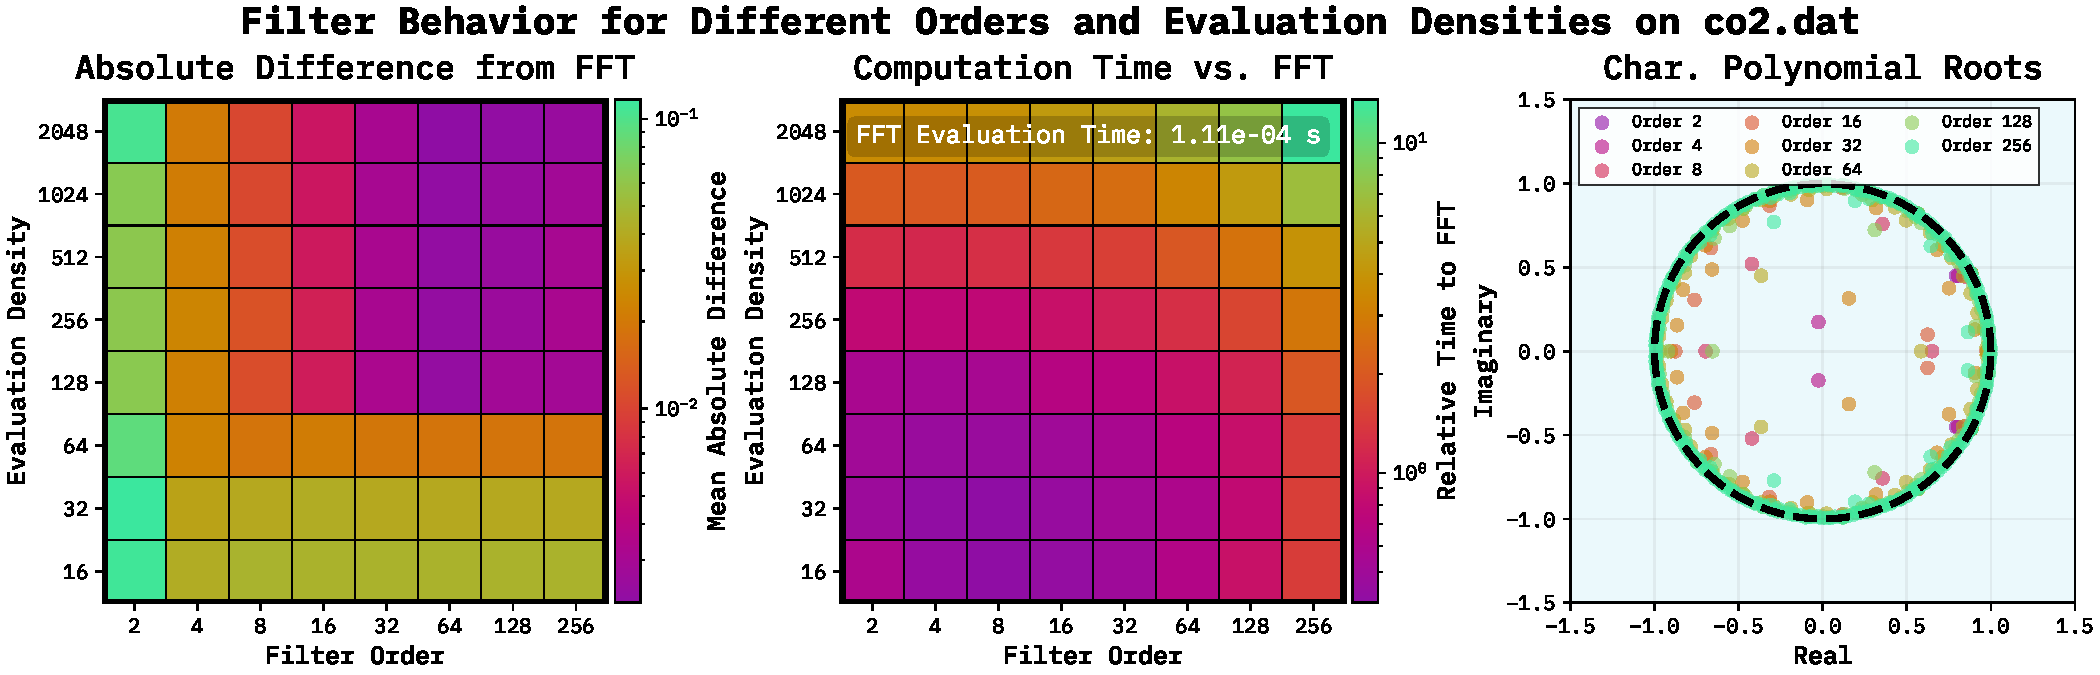
\includegraphics[width=0.95\textwidth]{../MaxEntropy/Images/order-density-co2.dat.pdf}
    \caption{The effects of filter order and evaluation density on the spectra of signal \texttt{co2.dat}.}
    \label{fig:order-3}
\end{figure}

The bright colors in combination with the bolded grid really remind me of a 80s dance floor, I hope the reader enjoys
the visual experience. The plots show that both the filter order and evaluation density have a significant impact 
on the spectra. One would naively expect that the absolute difference from the FFT spectra would decrease with 
increasing filter order, however that is not the case. In the plot for \texttt{val2.dat} and \texttt{val3} we see that the absolute
difference is lowest for the AR model of order $32$. The evaluation density has a lesser effect on the spectra, only comming 
into play when the density is very low and the peaks are not well resolved. In addition to absolute differences I've also plotted 
the computational times in comparison to the FFT spectra, where we can see that the AR model is comparable in speed 
to the FFT algorithm at the filter orders that yielded the best results. The right-most plot is there again for a 
sanity check to confirm that all of the roots are inside the unit circle. \\

It would be interesting to what the resolving power of an AR model is. What I mean by this is how close can to peaks 
be in the spectra for them to still be resolved. I did a little parameter scan for a couple of different values of filter 
order, peak separation distance and spectra evaluation density. The results of the scan are plotted in Figure 
\ref{fig:resolving-power}. The FFT spectra from the scan test signals are plotted in the Figure \ref{fig:resolving-power-test}.

\begin{figure}[H]
    \centering
    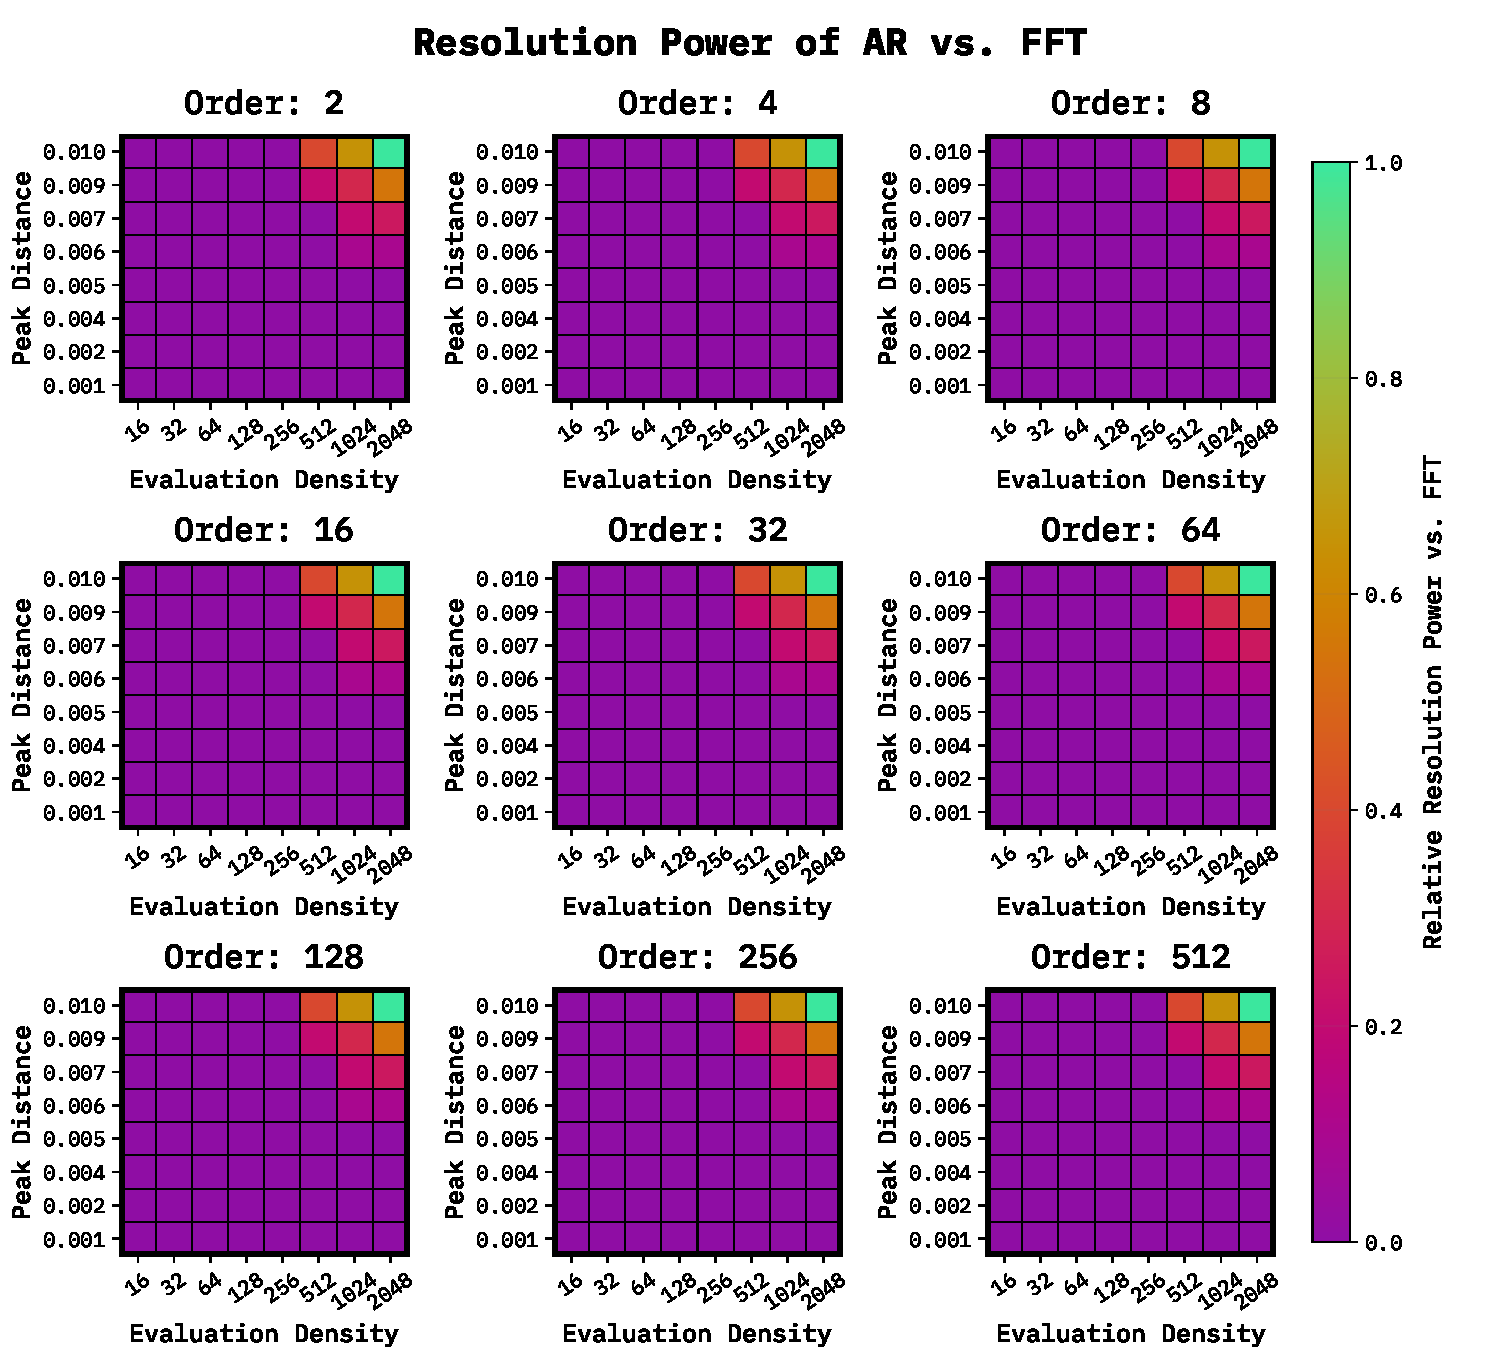
\includegraphics[width=0.95\textwidth]{../MaxEntropy/Images/s-res.pdf}
    \caption{The 'resolving power' of the AR model. Unresolved is colored in purple.}
    \label{fig:resolving-power}
\end{figure}

\begin{figure}[H]
    \centering
    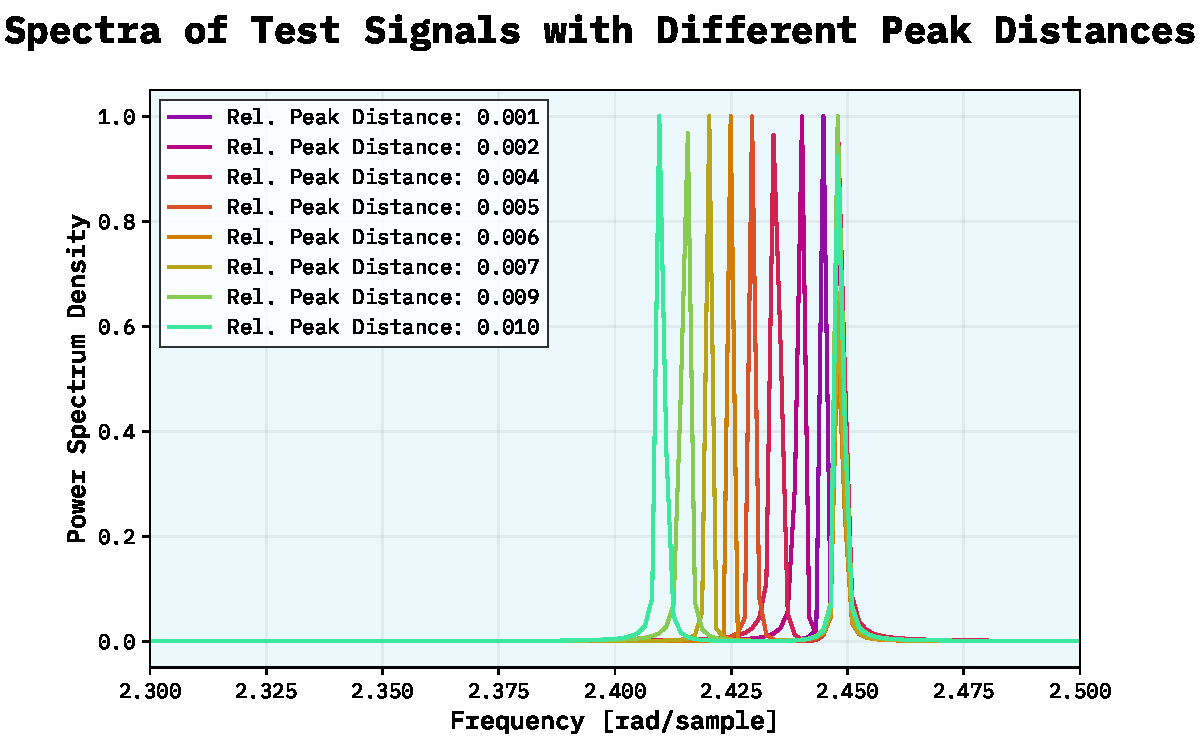
\includegraphics[width=0.8\textwidth]{../MaxEntropy/Images/test-spectra.pdf}
    \caption{The test spectra by FFT from the resolving power scan.}
    \label{fig:resolving-power-test}
\end{figure}

All resolving powers are compared to how far apart the peaks are in the FFT spectra. This plot represents one of my major disappointments
during this task in that, there is no dependence on the filter order, at least not in the range that I scanned. The results are 
the same for all filter orders. We can however see that in the range that I've provided only a small section of the parameter 
space contains peaks that actually managed to resolve. The majority of the peaks were not resolved to my great disappointment.
I inspected the spectra for any possible errors but they truly do seem to not resolve. The subset of the resultant spectra 
are plotted in Figure \ref{fig:resolving-power-spectra}.

\begin{figure}[H]
    \centering
    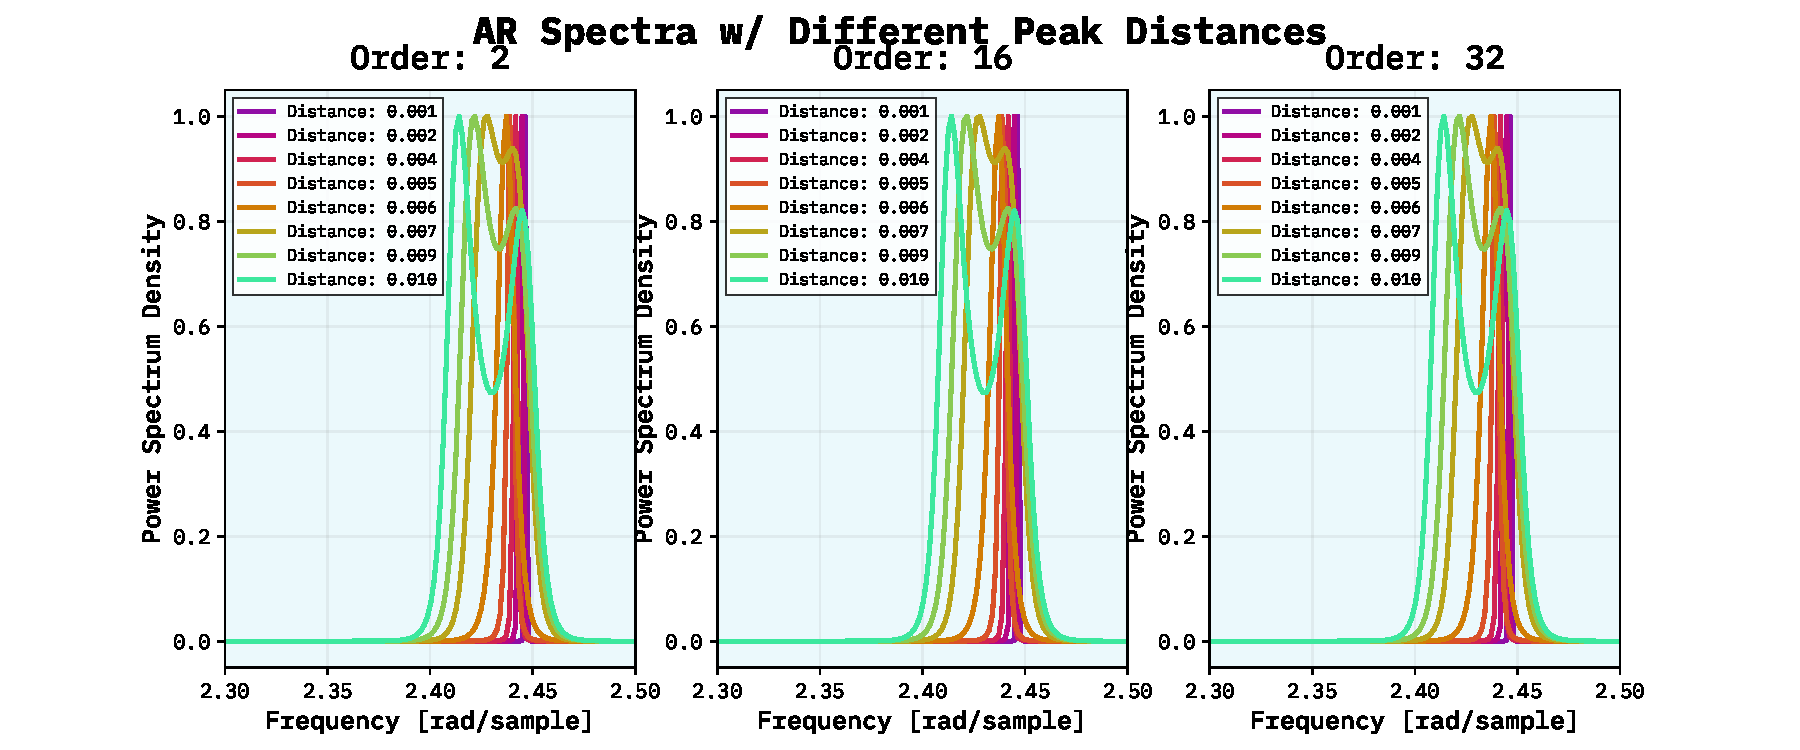
\includegraphics[width=0.95\textwidth]{../MaxEntropy/Images/ar-spectra.pdf}
    \caption{The subset of the spectra, where we can see most of the peaks are unresolved.}
    \label{fig:resolving-power-spectra}
\end{figure}

From this scan I was able to make a neat looking plot of execution times. It doesn't really have all that much value
now that we've seen that the filter order doesn't really matter. The plot is presented in Figure \ref{fig:execution-times}.

\begin{figure}[H]
    \centering
    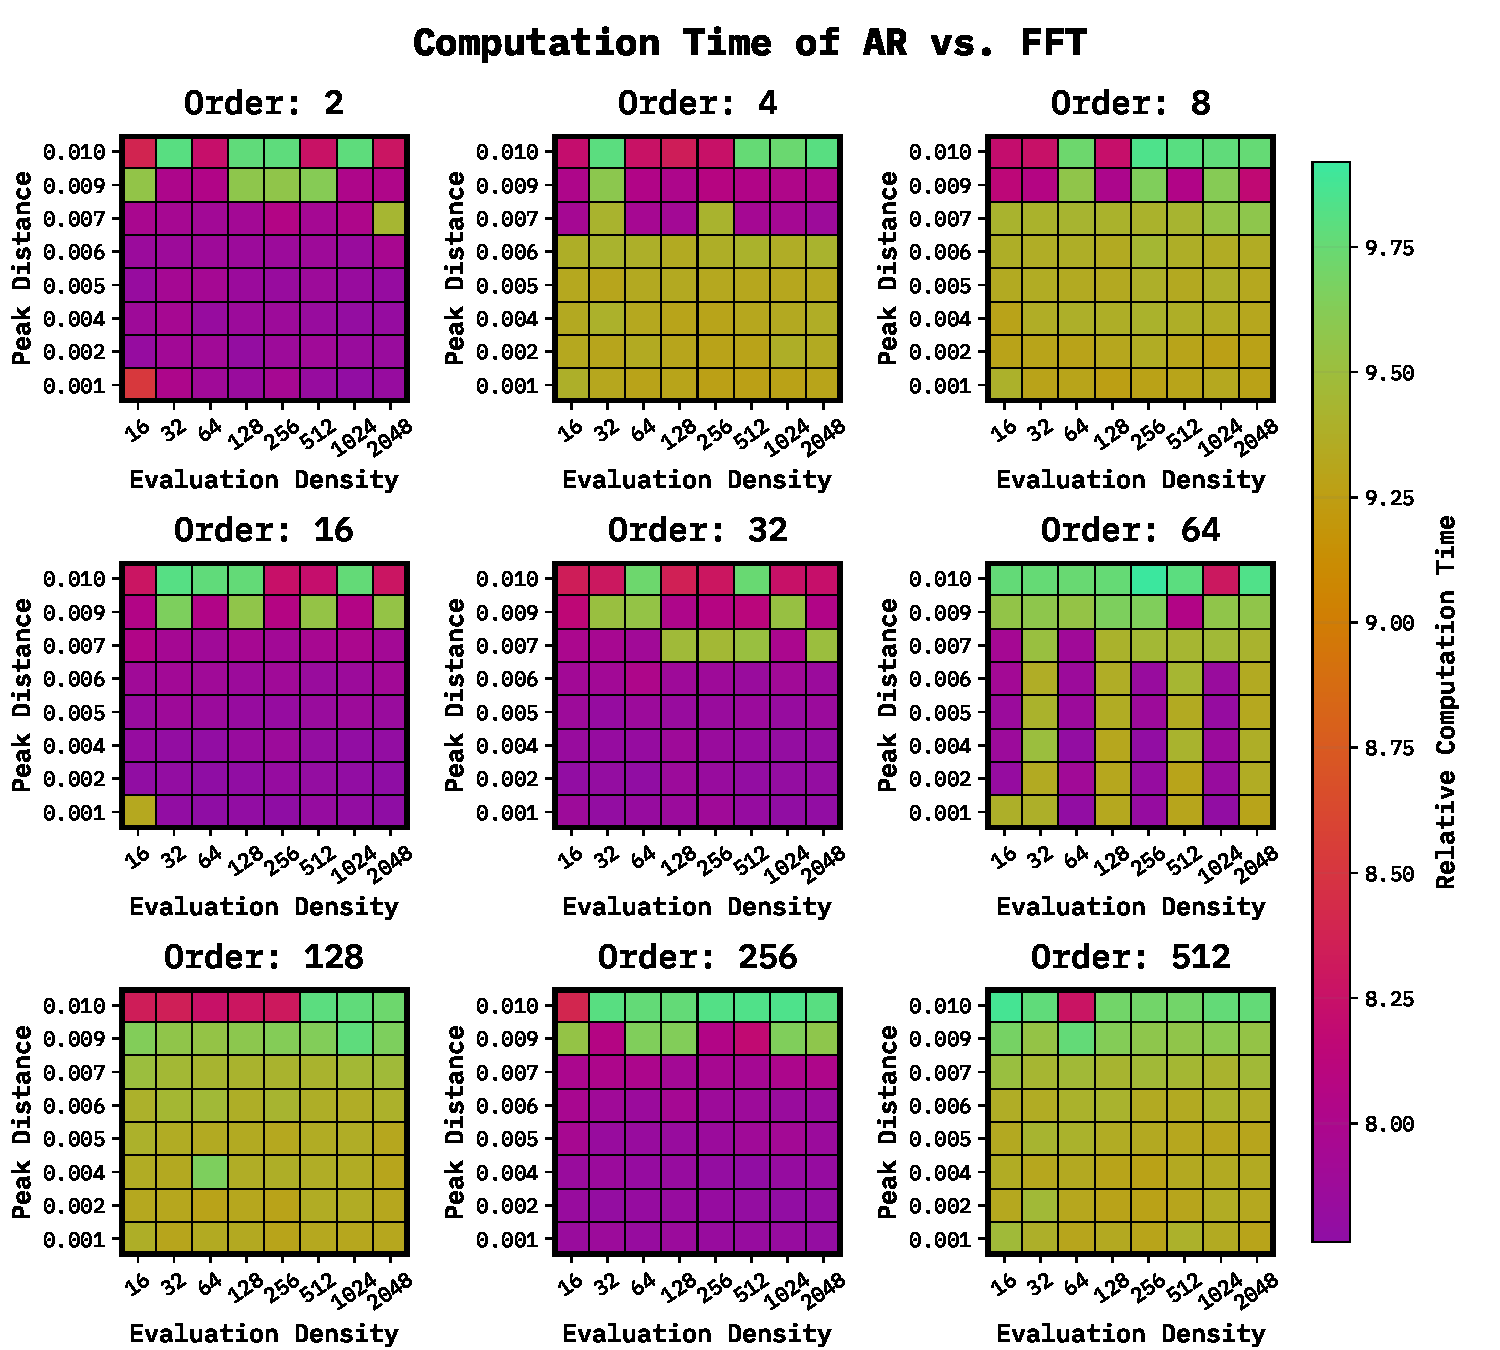
\includegraphics[width=0.8\textwidth]{../MaxEntropy/Images/time-res.pdf}
    \caption{The execution times of the AR model in comparison to the FFT algorithm.}
    \label{fig:execution-times}
\end{figure}

\subsection{Forecasting Signals}
As the instructions stated I used the AR model to forecast the various signals that were provided.. to varying 
degrees of success. The simpler signals from the first subtask were forecasted relatively well, excluding the fact that 
no matter what I did I could not get rid of an exponential decay of the overall amplitude of the forecasted signal. The results 
for the forecasted signals from the first subtask are plotted in Figure \ref{fig:forecast-1}, \ref{fig:forecast-2} and
\ref{fig:forecast-3}.

\begin{figure}[H]
    \centering
    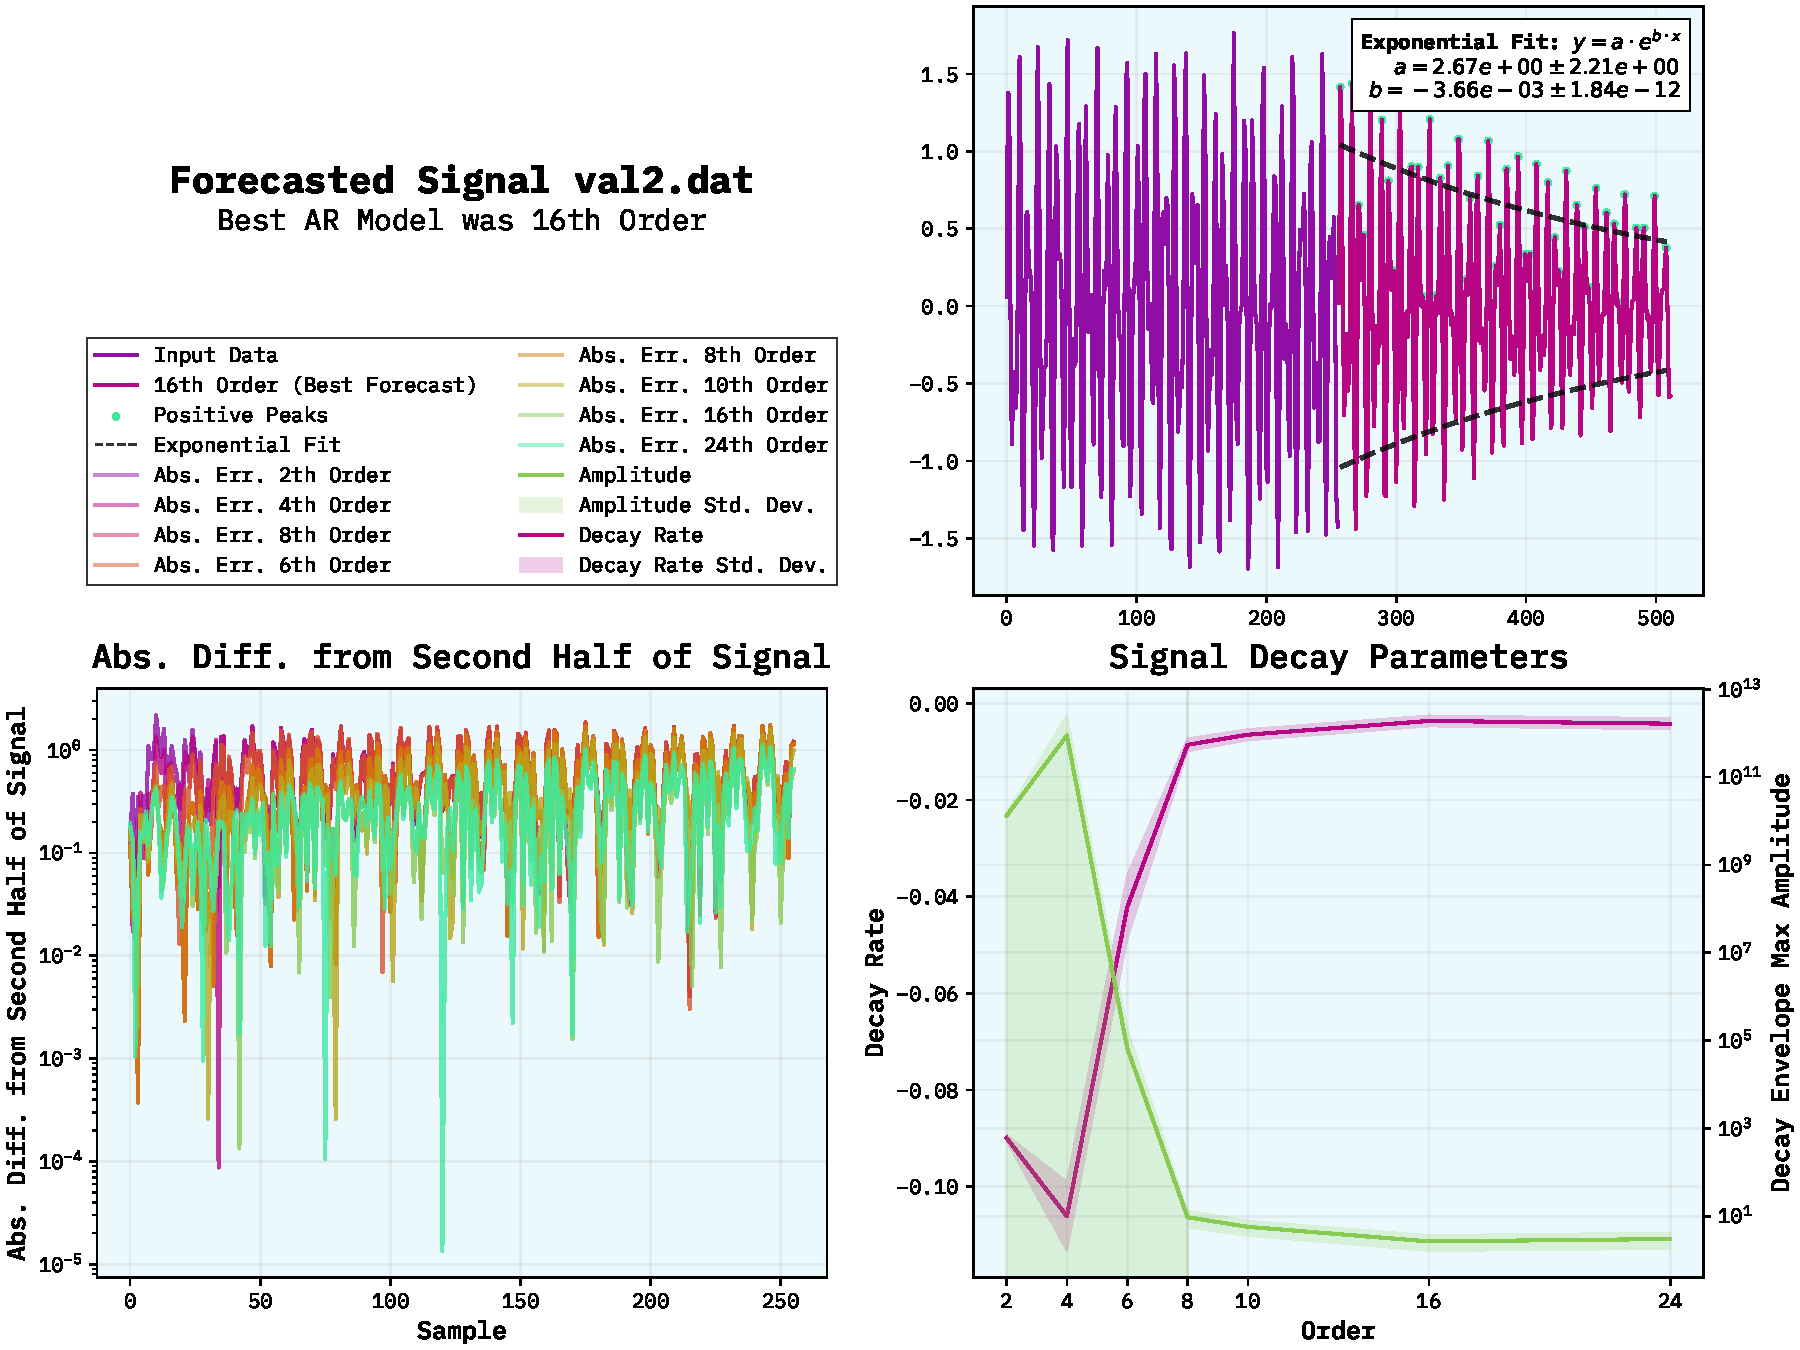
\includegraphics[width=0.8\textwidth]{../LinForecast/Images/forecast-val2.dat.pdf}
    \caption{The forecasted signal \texttt{val2.dat}.}
    \label{fig:forecast-1}
\end{figure}

\begin{figure}[H]
    \centering
    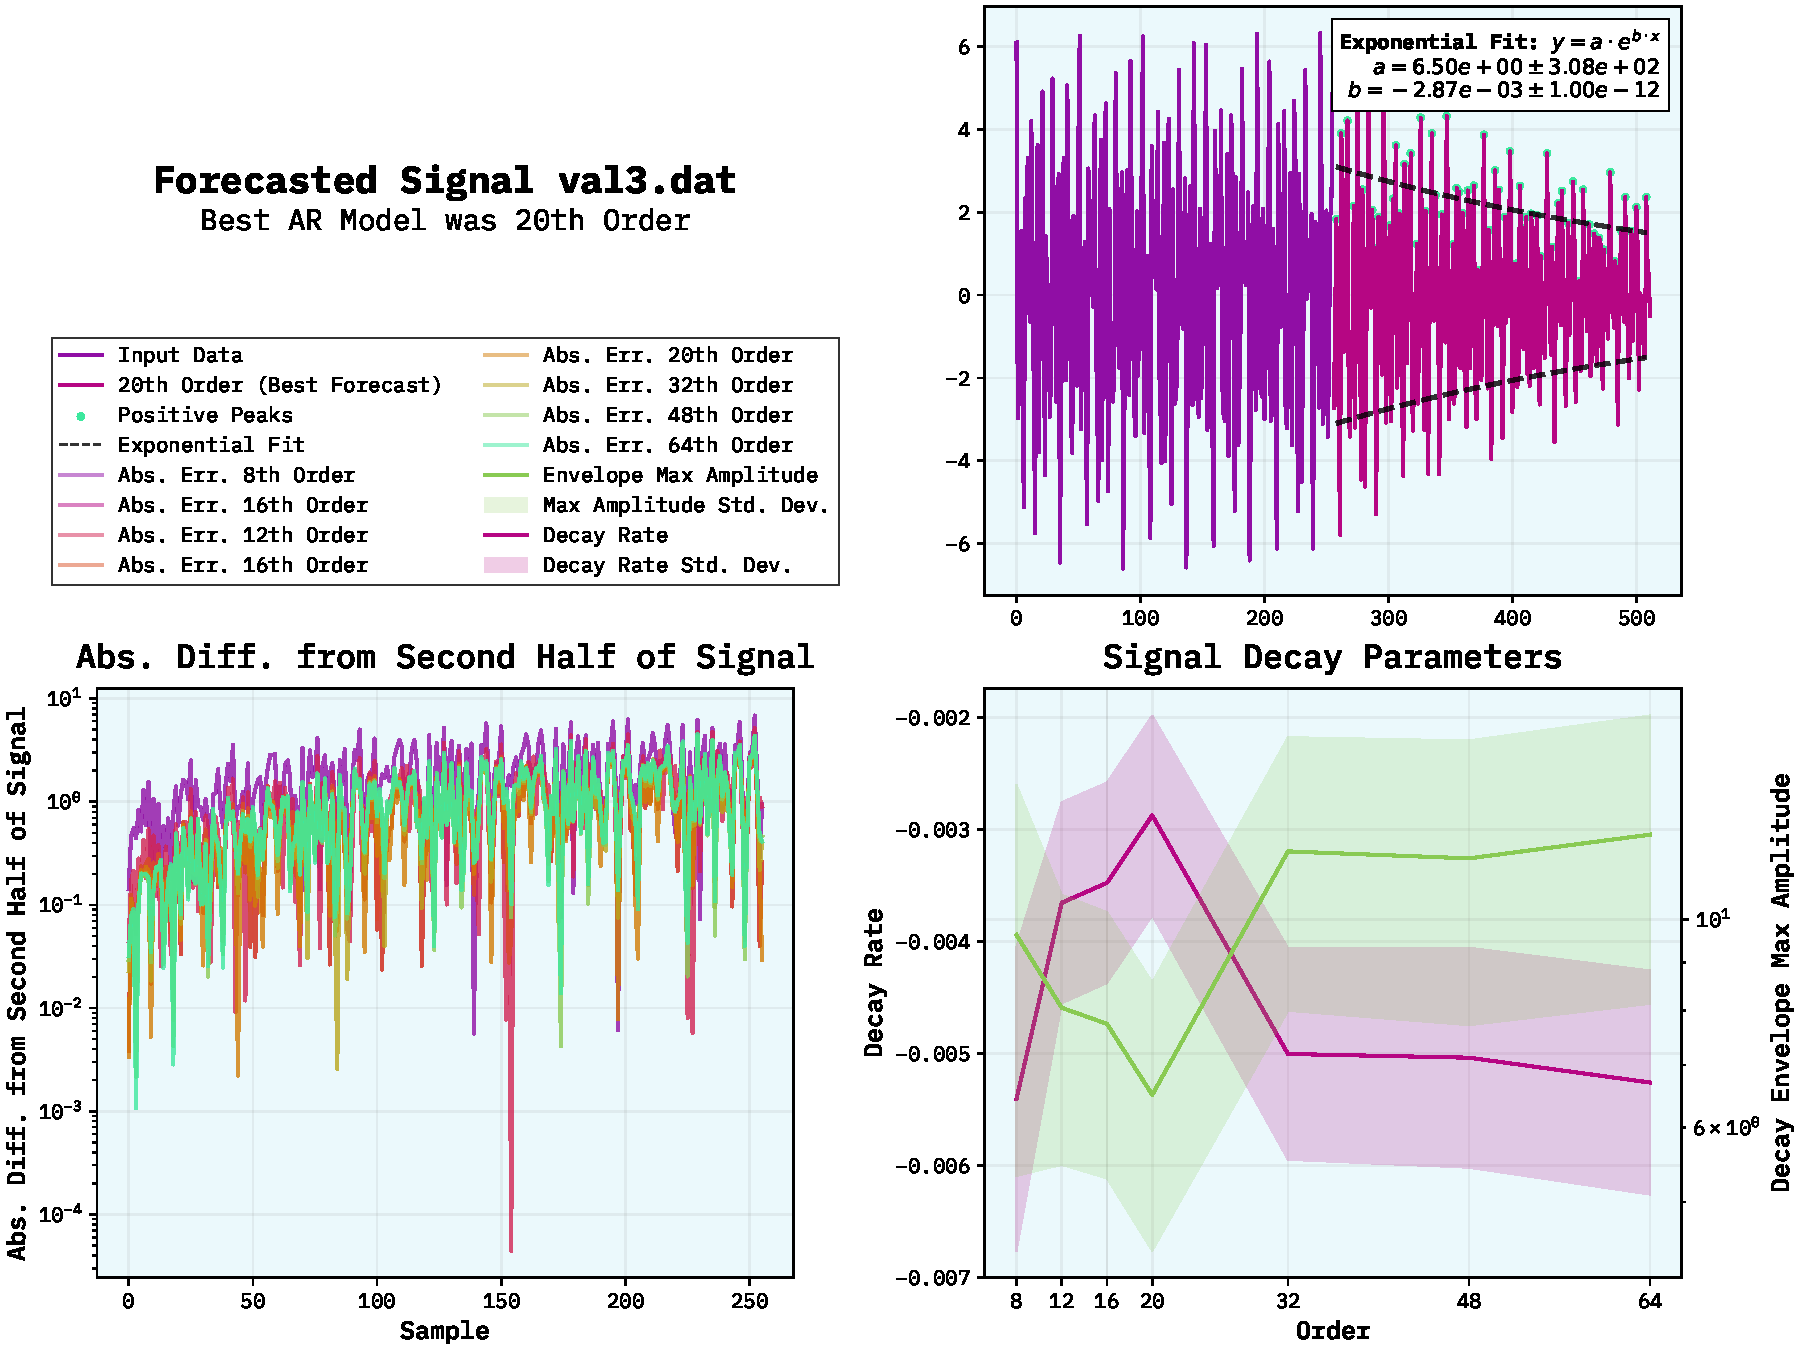
\includegraphics[width=0.8\textwidth]{../LinForecast/Images/forecast-val3.dat.pdf}
    \caption{The forecasted signal \texttt{val3.dat}.}
    \label{fig:forecast-2}
\end{figure}

\begin{figure}[H]
    \centering
    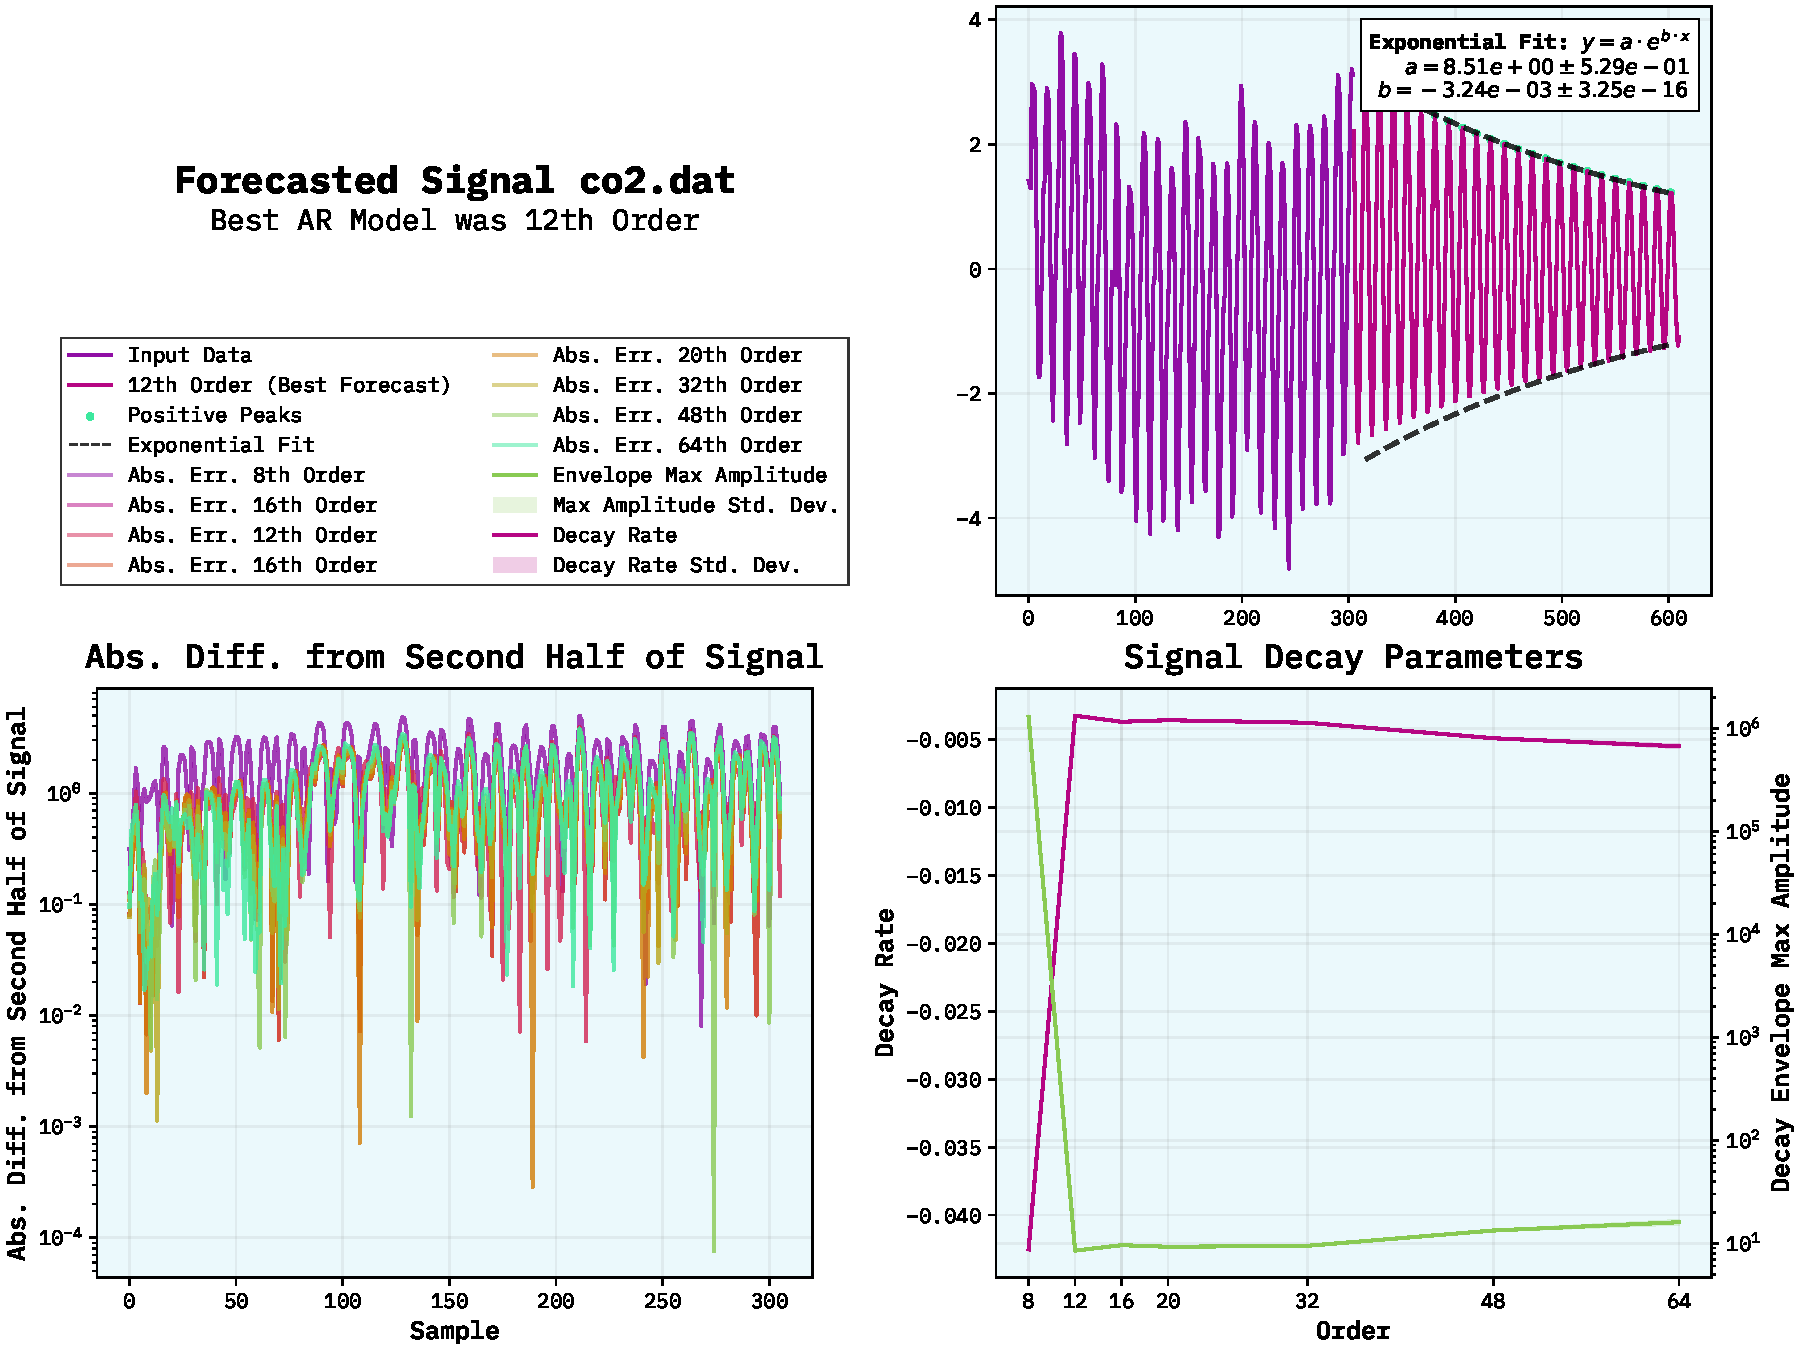
\includegraphics[width=0.8\textwidth]{../LinForecast/Images/forecast-co2.dat.pdf}
    \caption{The forecasted signal \texttt{co2.dat}.}
    \label{fig:forecast-3}
\end{figure}

Since I was not able to remove the exponential decay trend I fitted an exponential decay and tried to find the order 
of AR model that would provide the smallest decay rate. The upper-right plot contains the best case result for the 
forecast of the signals. Where we can see that all have been predicted reasonably well. The further we go in time 
the worse the forcasts become which can also be seen on the plots of the absolute distance from the control signal, 
which is made from the second half of the data. Pattern and shape-wise the forecasted signals seem very similar to the 
control signals. The only part of the forecast I find lacking (besides the decay) is for the \texttt{co2.dat} signal 
where the forecasted signal lacks the overall larger oscillations that still seem to be present in the detrended signal. \\

The forecasted signals from the second subtask were definitely more challenging and I'm less happy with the results I was 
able to produce. The results are plotted in Figure \ref{fig:forecast-4}, \ref{fig:forecast-5} and \ref{fig:forecast-6}.

\begin{figure}[H]
    \centering
    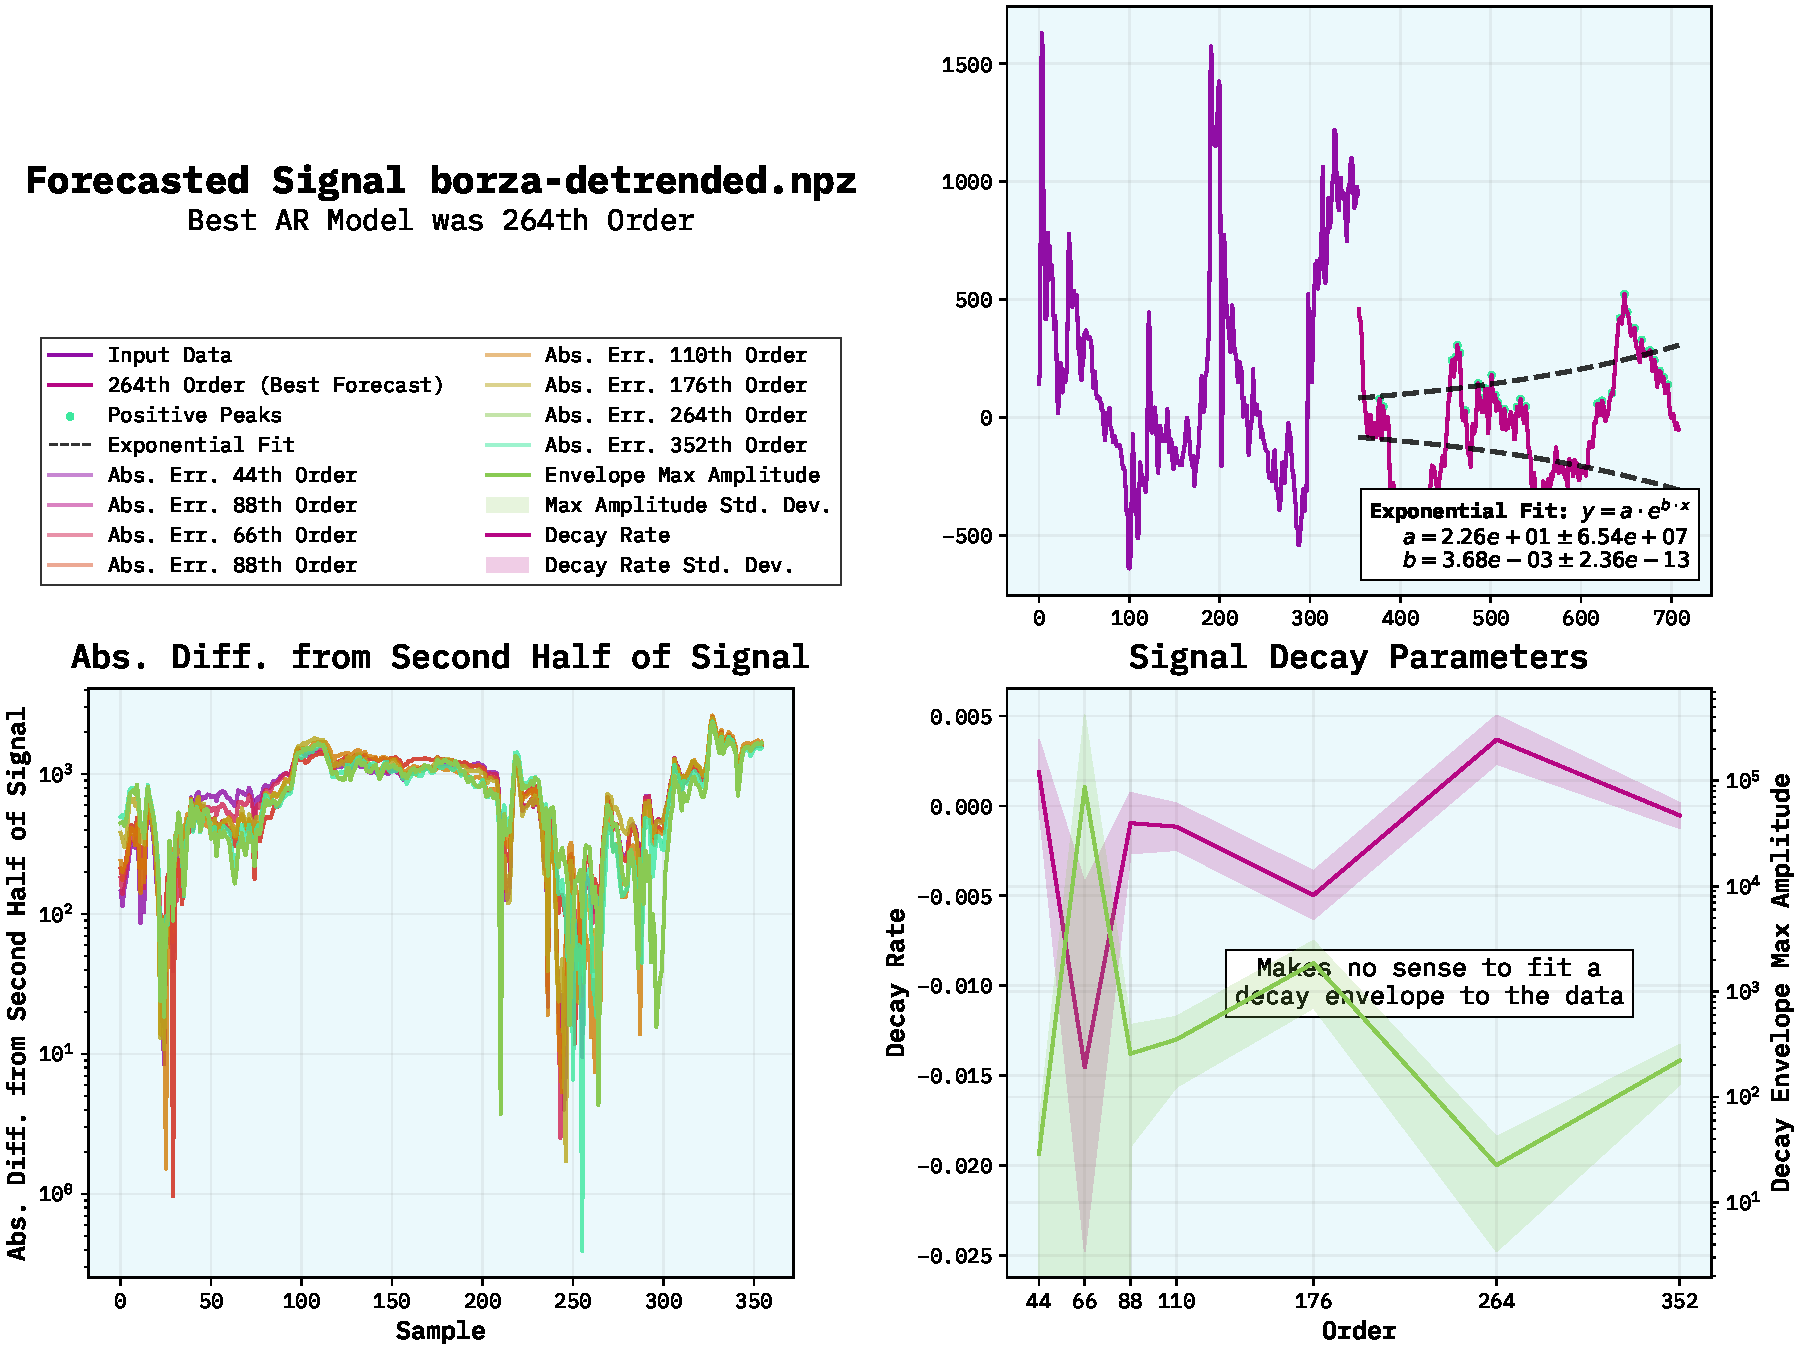
\includegraphics[width=0.8\textwidth]{../LinForecast/Images/forecast-borza-detrended.npz-lin.pdf}
    \caption{The forecasted signal \texttt{borza.dat}.}
    \label{fig:forecast-4}
\end{figure}

\begin{figure}[H]
    \centering
    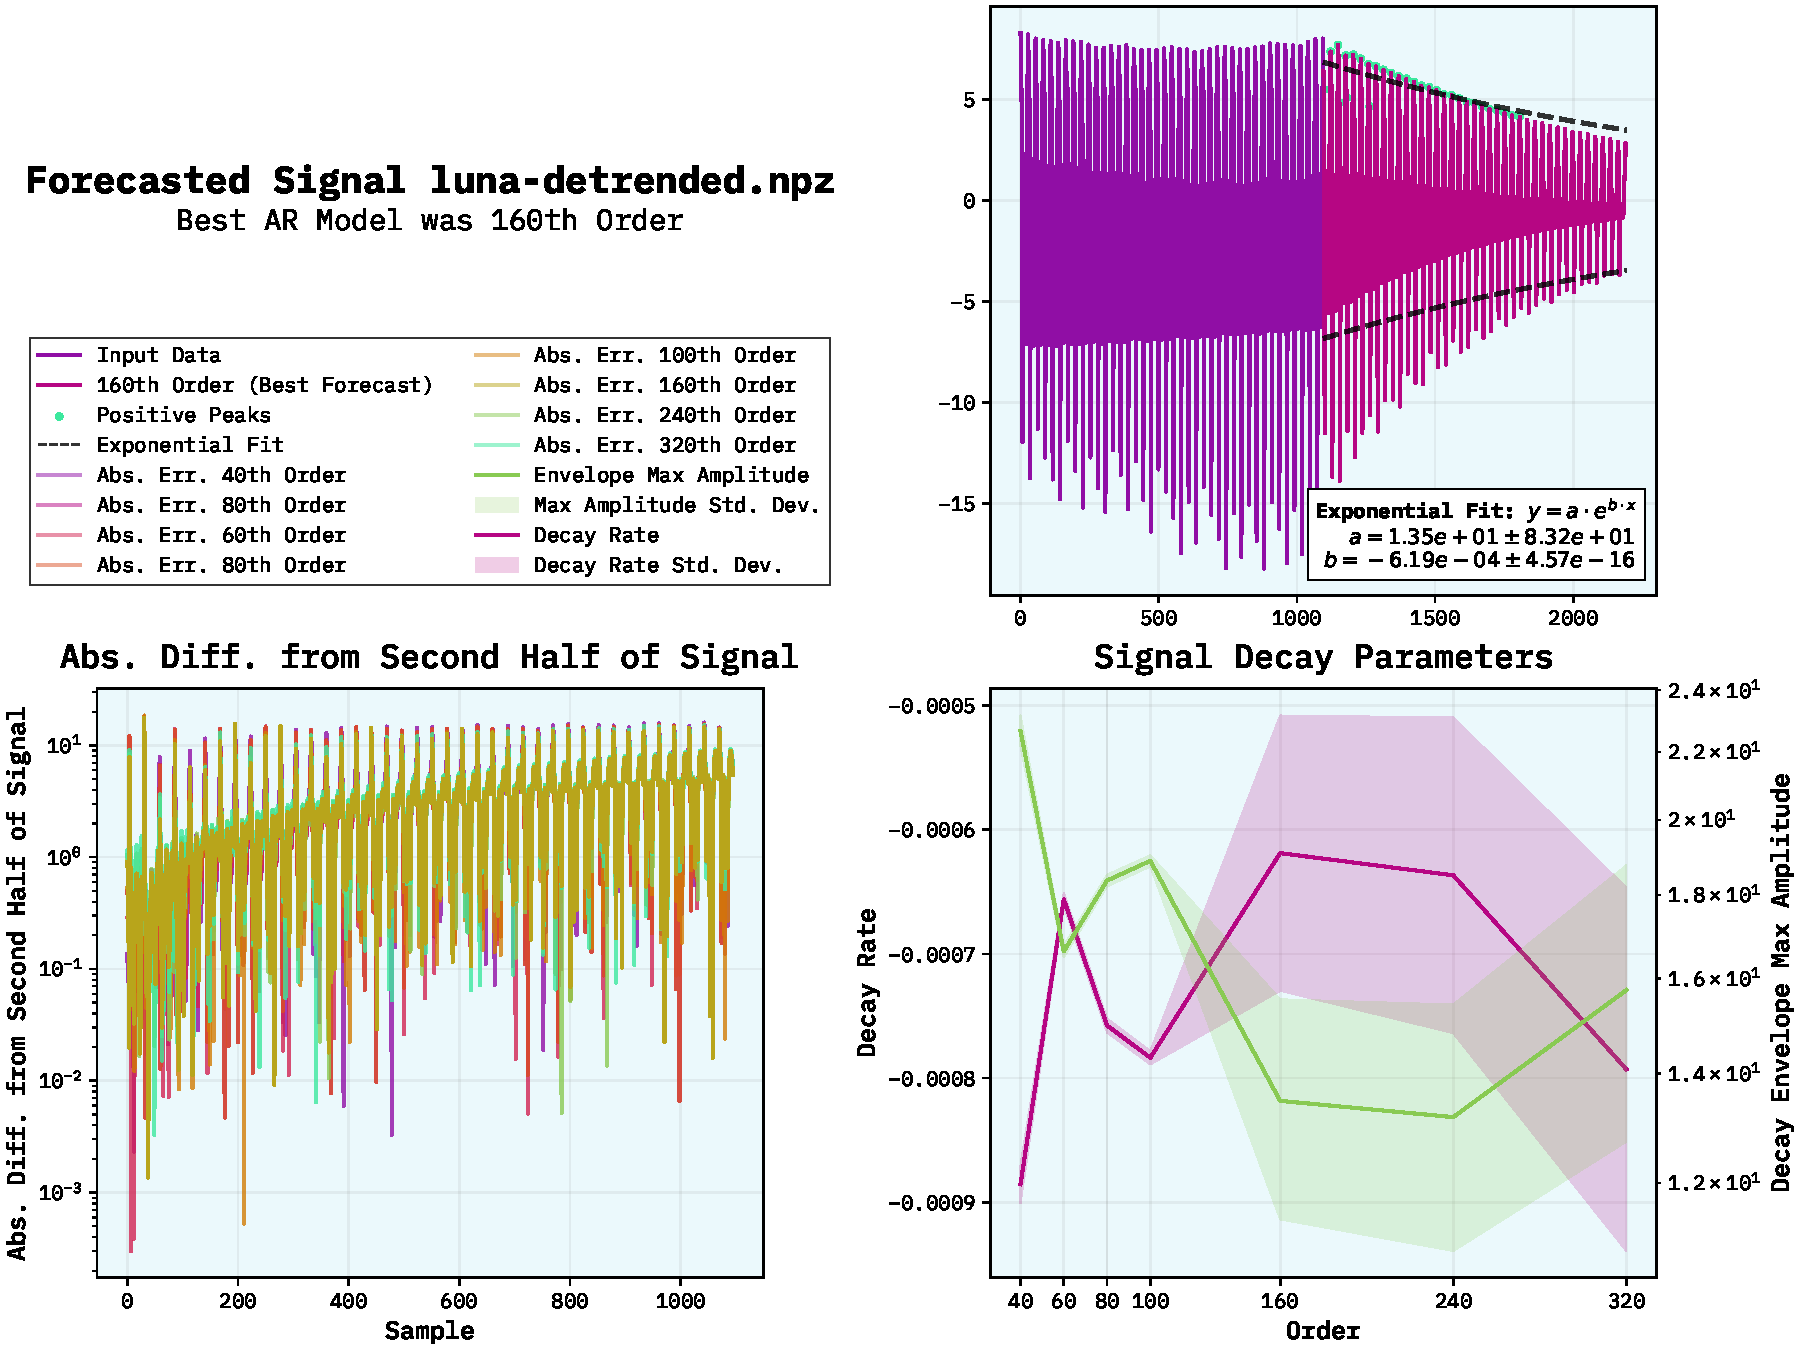
\includegraphics[width=0.8\textwidth]{../LinForecast/Images/forecast-luna-detrended.npz.pdf}
    \caption{The forecasted signal \texttt{moon.dat}.}
    \label{fig:forecast-5}
\end{figure}

\begin{figure}[H]
    \centering
    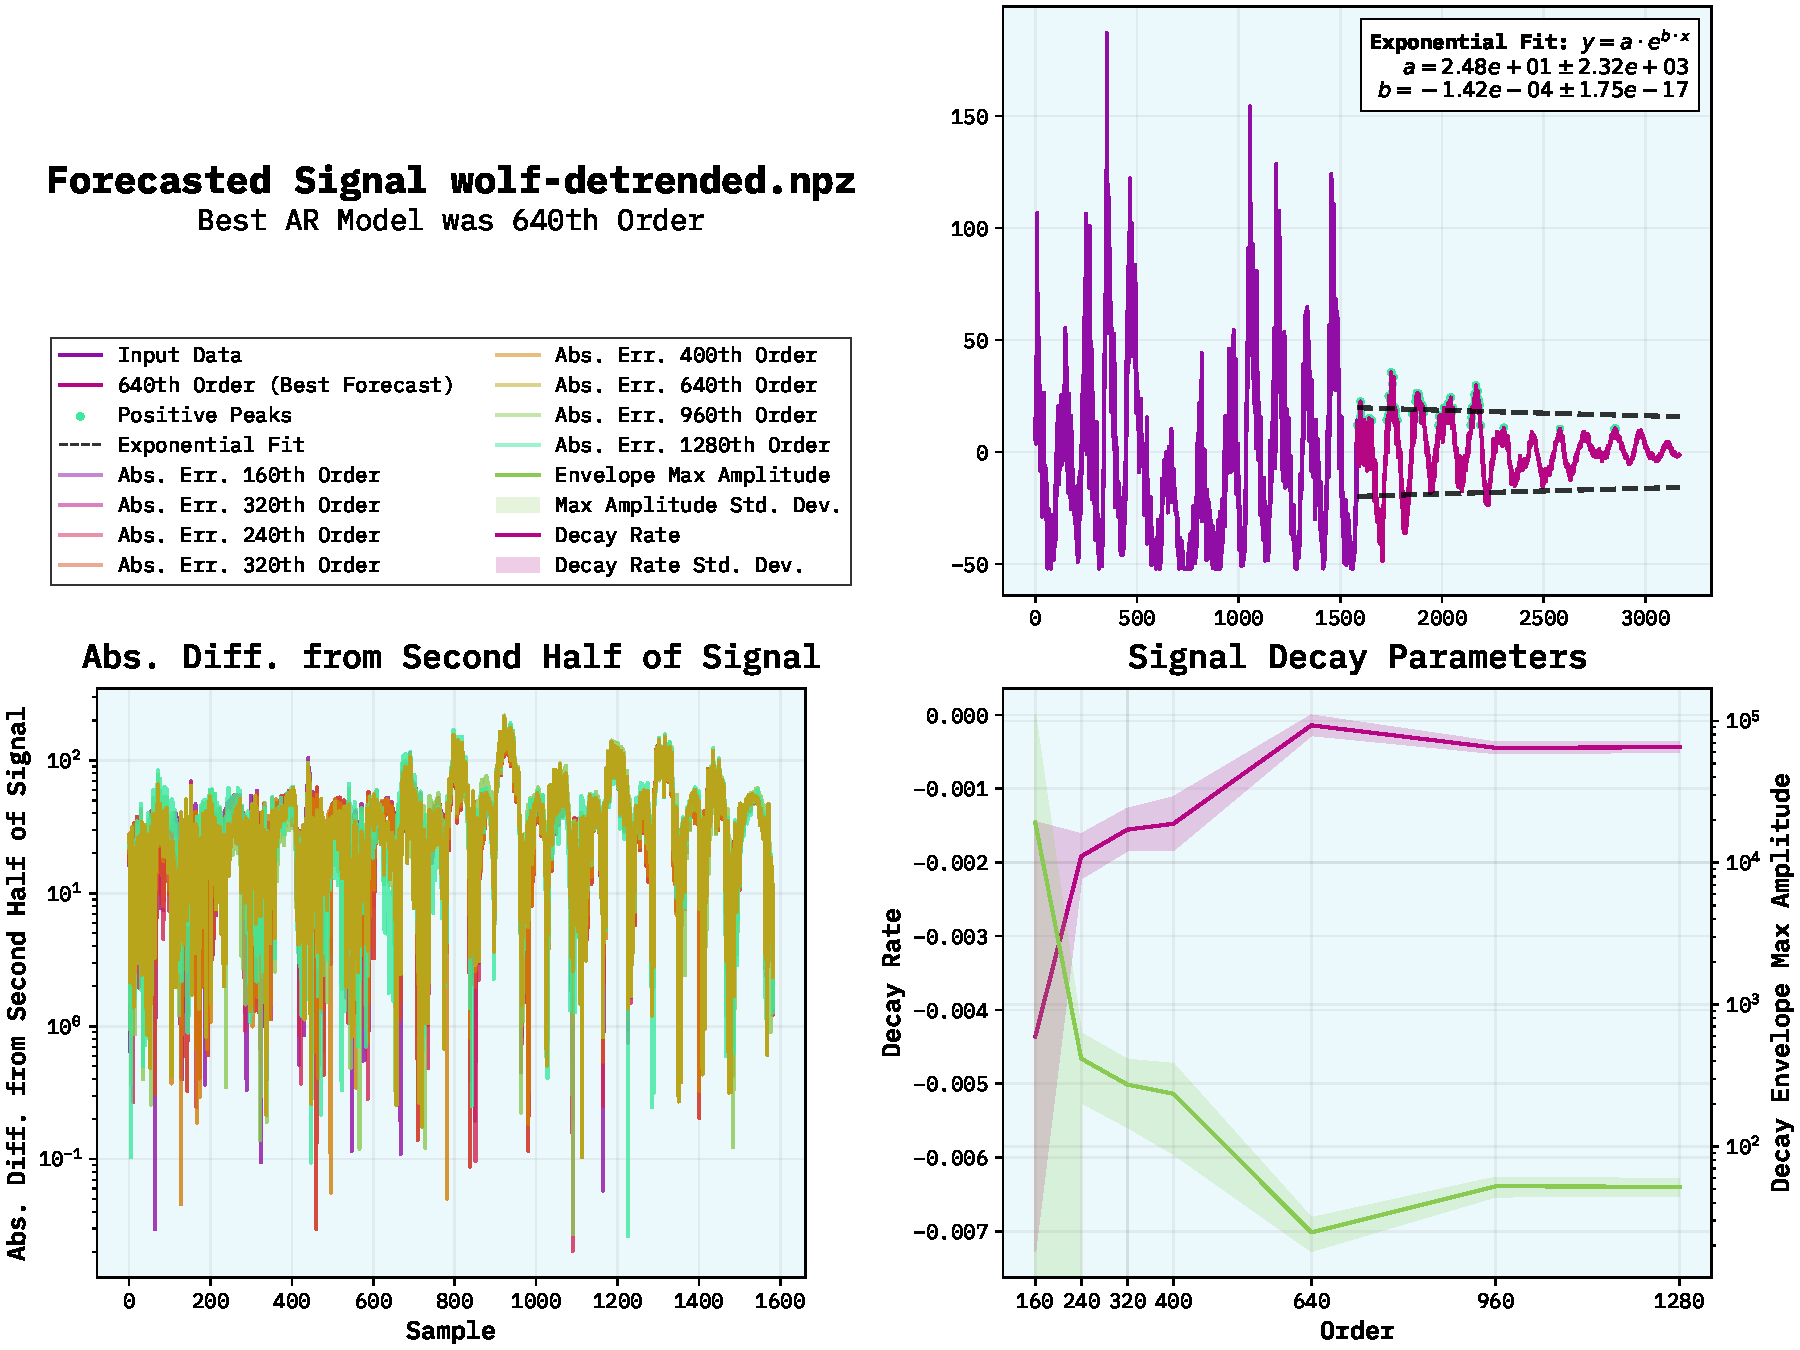
\includegraphics[width=0.8\textwidth]{../LinForecast/Images/forecast-wolf-detrended.npz.pdf}
    \caption{The forecasted signal \texttt{sunspot.dat}.}
    \label{fig:forecast-6}
\end{figure}

I'd like to make a note that the signal \texttt{luna.dat} was composed of two coordinates, the Right Ascension and
Declination of the moon. For simplicity I combined these two with the root of the sum of the squares. Out of all the 
signals provided in the second dataset I think the Wolf sunspot numbers were forecasted the best. There seems to be relatively
sensible continuity in the forecasted signal and again we can fit a somewhat weak exponential decay trend to the forecast. We can also 
clearly see from the plotted parameters of the decay fit for various AR model orders that the decay rate is smallest somewhere in the 
middle. The absolute worst results were for the stock value signal. Even though I tried hard to remove any existing trends 
the forecasted signal is not continuous as it contains a large gap between the last point of the input signal and the first forecasted 
point. The shape seems to be somewhat similar to what we would expect except that when having a look at the absolute difference 
we find that it is absolutely abysmal, reaching values of $10^3$. Fitting an exponential decay here also made little sense but 
I did it anyway, only to find that the best decay rate was actually positive which really does not make sense. The moon signal 
was forecasted relatively well I suppose. Due to the asymmetry of the signal (despite the detrending) the forecasted signal 
is biased towards the positive values and with errors towards the end of the forecast reaching above $10^0$, I'm not sure 
that this forecast would be the most useful. \\

Due to being strapped for time I was not able to do any further analysis on the forecasted signals, barring a quick look at how 
adding noise to the input signal affects the forecast. I evaluated this for only the simplest signal {val2.dat}, for three different 
values of noise standard deviation. The results are plotted in Figures \ref{fig:noise-1}, \ref{fig:noise-2} and \ref{fig:noise-3}.

\begin{figure}[H]
    \centering
    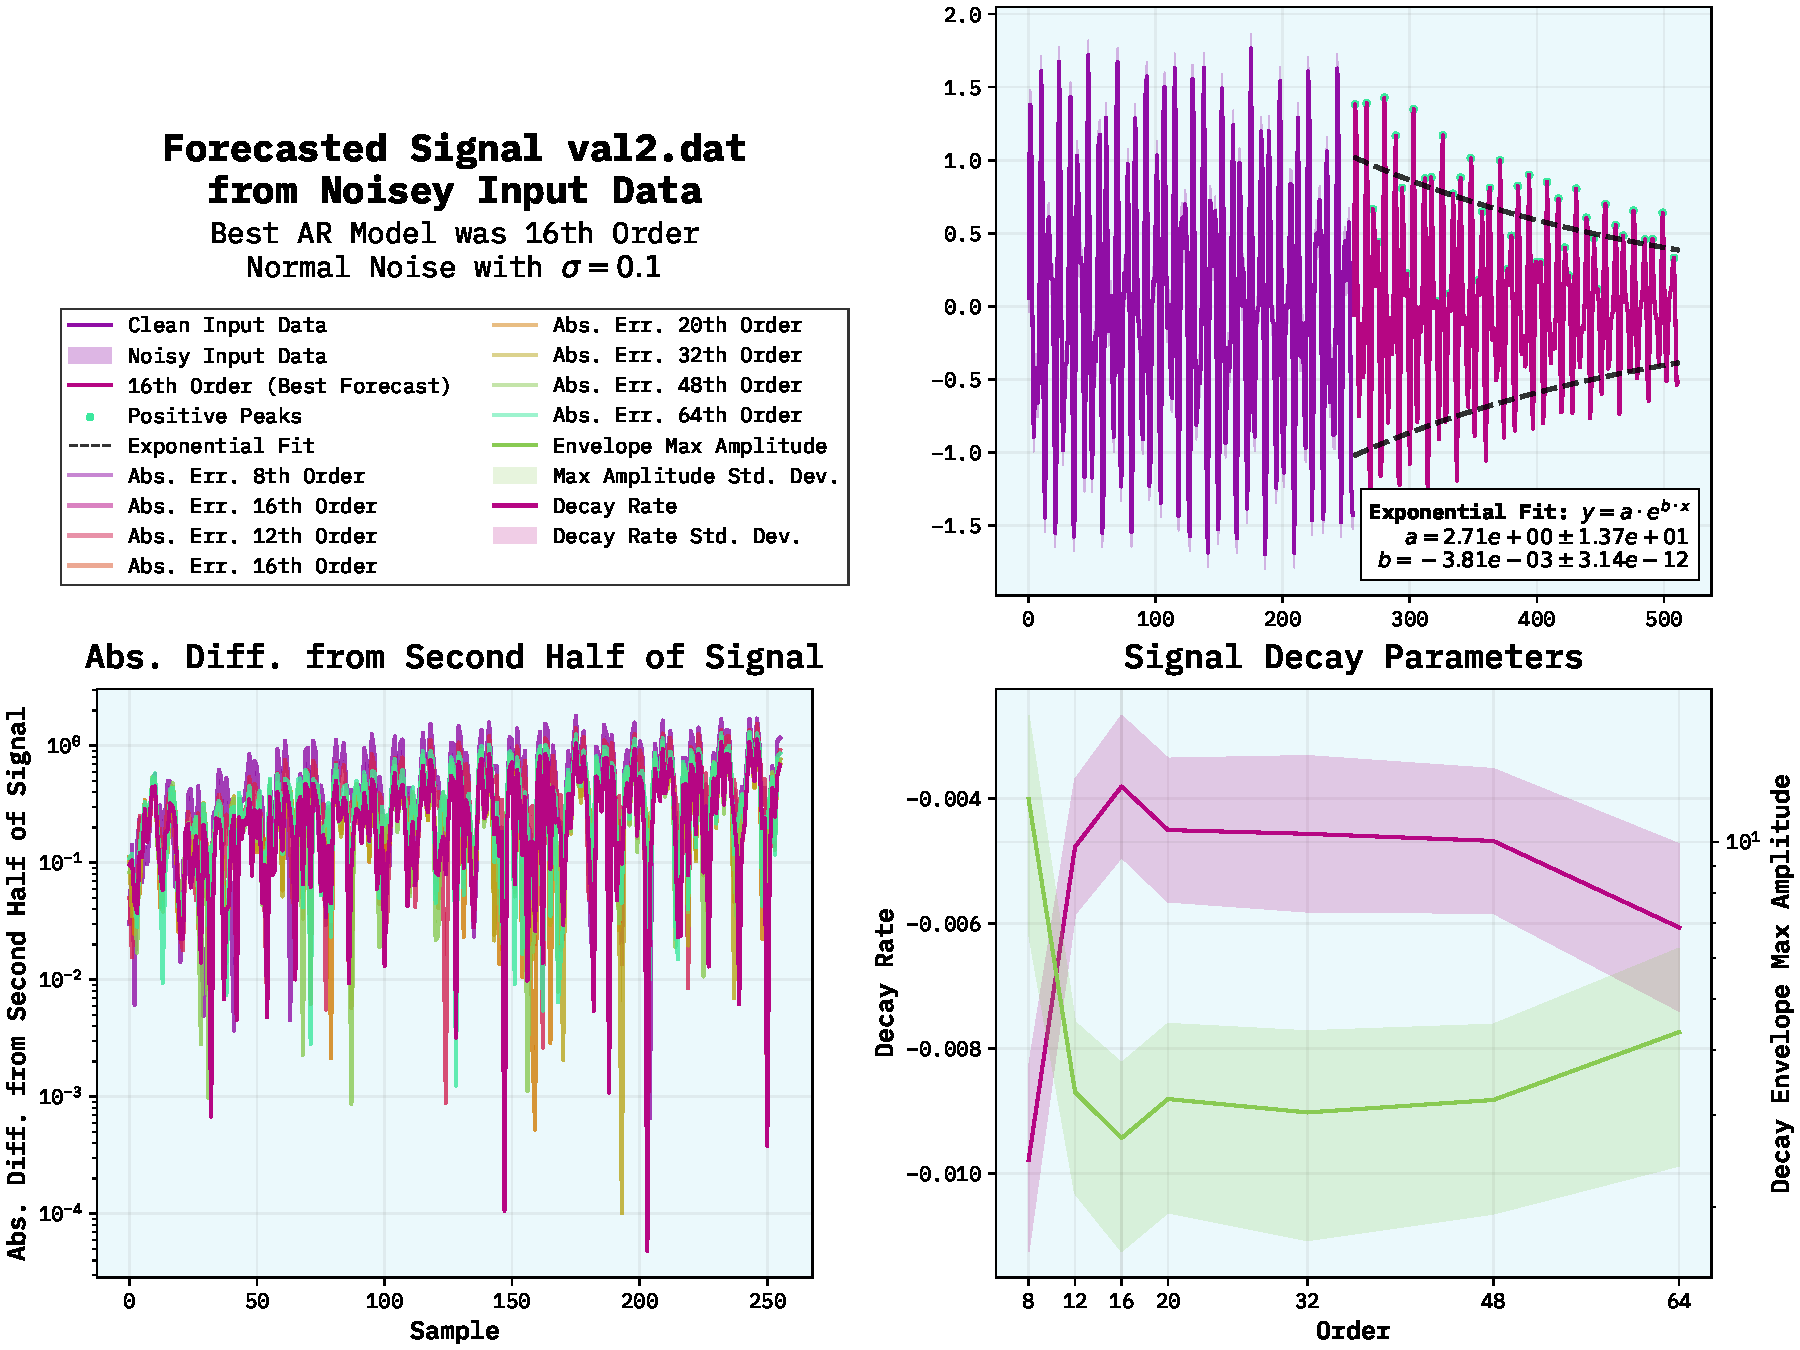
\includegraphics[width=0.8\textwidth]{../LinForecast/Images/noisey-forecast-val2.dat-0.1.pdf}
    \caption{The forecasted signal \texttt{val2.dat} with added noise of standard deviation $0.1$.}
    \label{fig:noise-1}
\end{figure}

\begin{figure}[H]
    \centering
    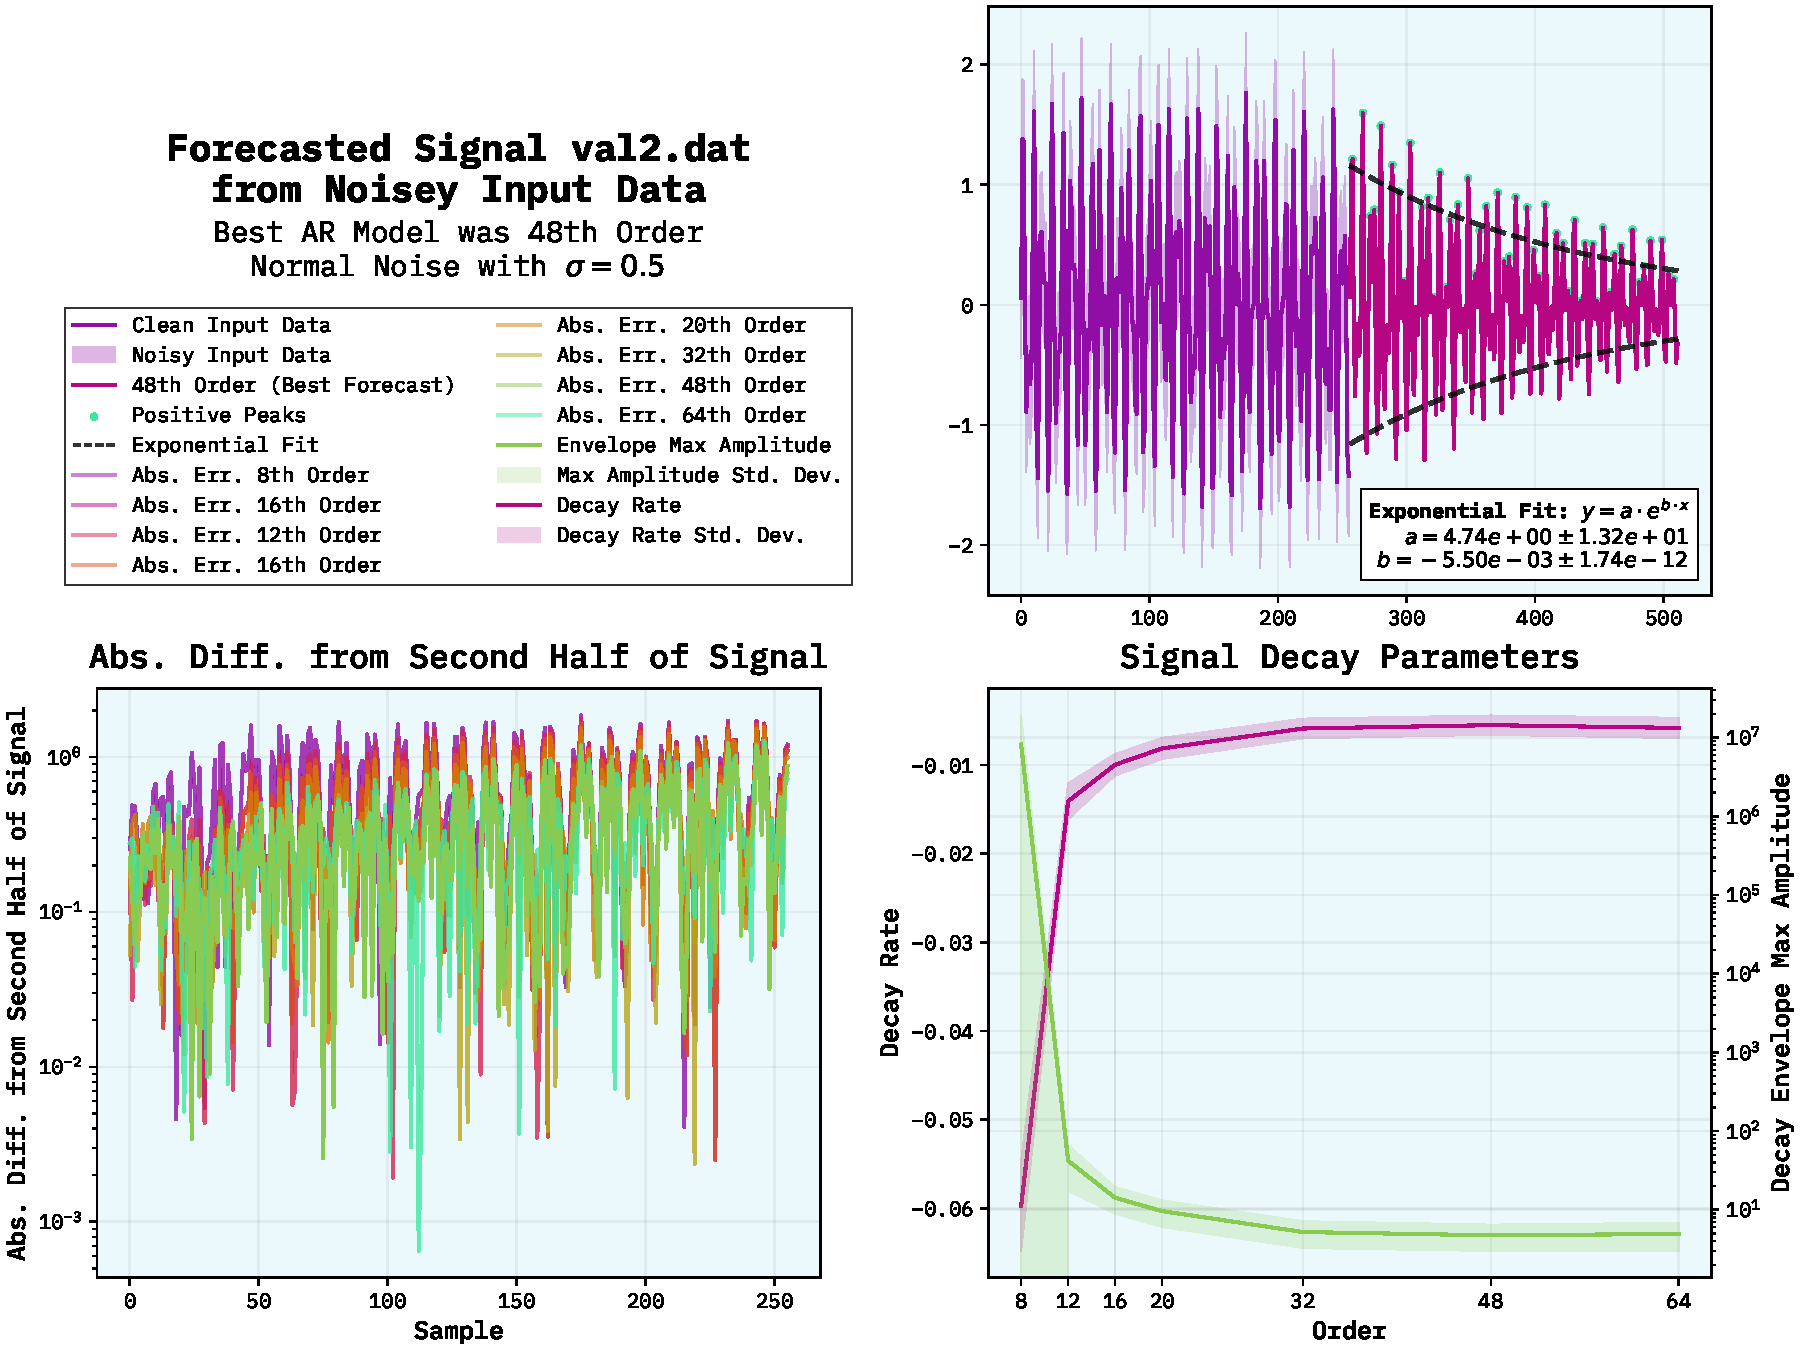
\includegraphics[width=0.8\textwidth]{../LinForecast/Images/noisey-forecast-val2.dat-0.5.pdf}
    \caption{The forecasted signal \texttt{val2.dat} with added noise of standard deviation $0.5$.}
    \label{fig:noise-2}
\end{figure}

\begin{figure}[H]
    \centering
    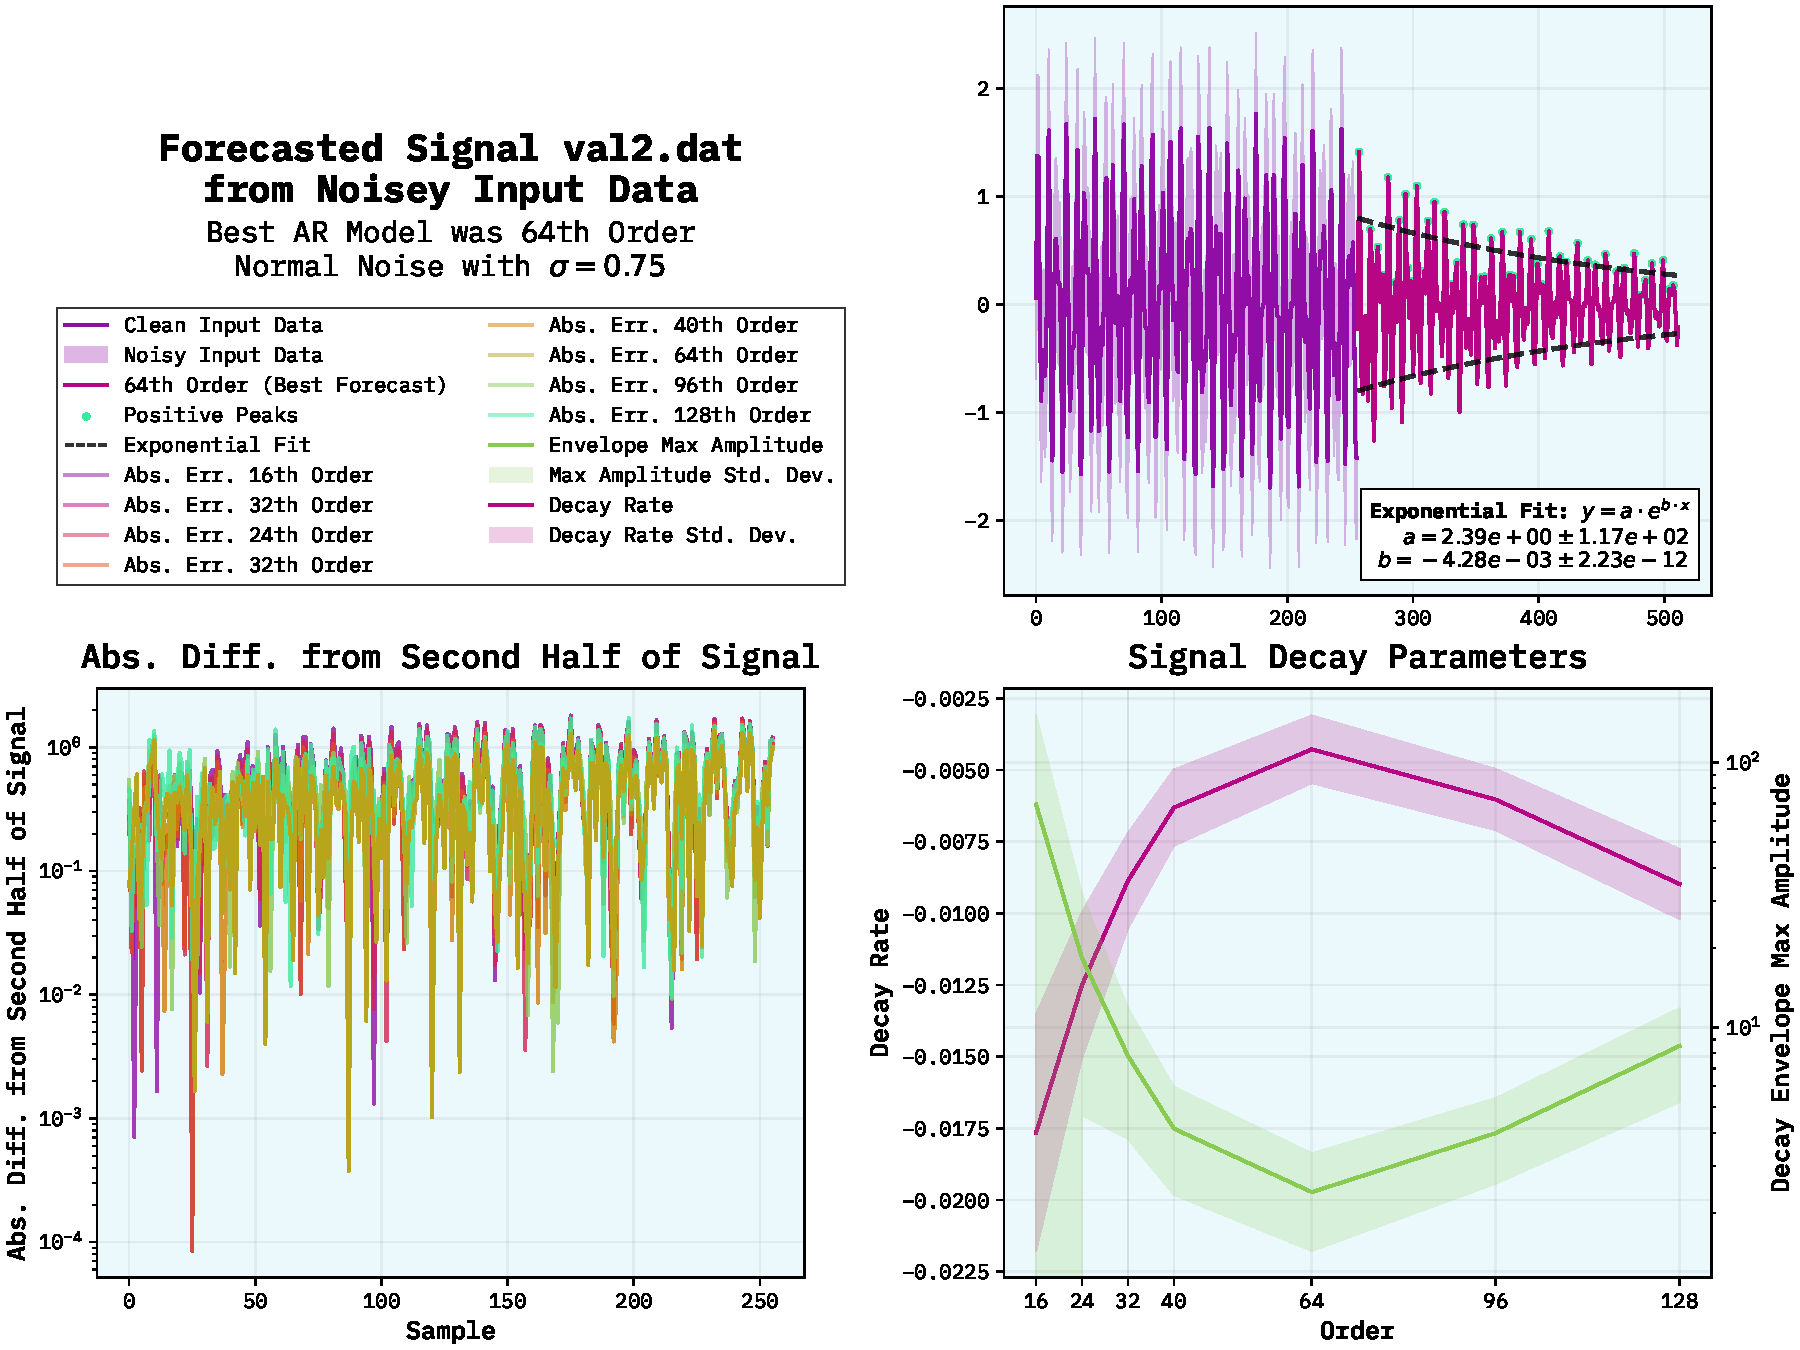
\includegraphics[width=0.8\textwidth]{../LinForecast/Images/noisey-forecast-val2.dat-0.75.pdf}
    \caption{The forecasted signal \texttt{val2.dat} with added noise of standard deviation $0.75$.}
    \label{fig:noise-3}
\end{figure}

The trend I spotted with the addition of increasing noise is that the best AR model order for the forecast rises with 
the increasing standard deviation of the noise. In all examples the forecasted signal looks correct to the signal before it 
but really lacks in amplitude despite my best efforts. We can see that a stronger value of noise really diminishes the amplitude 
of the forecasted signal and with that the absolute difference from the control signal rises. Overall even with a 
$\sigma = 0.75$ the forecasted signal still seems to match the shape of the input signal. Perhaps there exists a better way
to adjust for the exponential decay. Our professor included an article called \textit{Why Yule-Walker Should Not Be Used 
for Autoregressive Modeling} \cite{no-yw} which states that the Yule-Walker method is not the best method for AR model
fitting and suggests a look at the Burg method, which will unfortunately have to be left for another time.


\section{Conclusion and Comments}
Overall I'm happy with the results that I was able to produce however I do feel that I could have done more. Especially 
for forecasting of signals where half of the results I got were not really satisfactory. One thing I'd definitely take a look 
at had I the time is the Burg method for AR model fitting. I'd also maybe like to do some more meta-studies on AR model forecasting, eg.
how far into the future is it possible to reasonably forecast a signal. The task also lacks any really original data to 
analyize which is a bit of a shame. On to the last task! Oh and whoever thought of exporting dates firstly in the format
\texttt{JUN19}, and secondly for multiple years, cause me quite the headache.

% Add references
\newpage
\bibliographystyle{unsrt}
\bibliography{mod112}

% End document
\end{document}
